\chapter{Ergebnisse}
\label{Ergebnisse}

In den folgenden Abschnitten werden die Ergebnisse dieser Arbeit aufgezeigt und erklärt.
Sie sind unterteilt in die drei Evaluations-Strategien, die in Abschnitt \ref{sec:Evaluation} erläutert wurden: Analyse der Rohdaten, bayes'sche Analyse und graphische Evaluation.
Zur Vereinfachung wird die konstante Rekombinationsrate kurz \glqq Konstant\grqq\space genannt, die linear fallende Rekombinationsrate \glqq Clegg \grqq\space und die Rekombinationsrate mit der One-Fifth Regel \glqq One-Fifth\grqq.

\section{Ergebnisse Rohdatenanalyse}
\label{sec:ergebnisseRohdaten}

Die Analyse der Rohdaten besteht aus zwei Teilen.
Die Ergebnisse der Hyperparameteranalyse werden für Parity und Keijzer näher betrachtet.
Es werden dabei folgende Werte für jede CGP-Konfiguration aufgezeigt:\\
\textbf{Anzahl der Rechenknoten:} Anzahl der Rechenknoten in jedem Chromosom des CGP-Modells\\
\textbf{$\lambda$ (Nachwuchs):} Anzahl der Nachwuchs-Chromosomen in jeder Generation; $\lambda$-Wert in der ($\mu$+$\lambda$)-ES\\
\textbf{Start-Rekombinationsrate:} Rekombinationsrate bei der Initialisierung; nur relevant für die konstante Rekombinationsrate und die One-Fifth Regel (linear fallende Rekombinationsrate wird mit 0,9 initialisiert)\\
\textbf{Delta Rekombinationsrate:} Dieser Wert wird bei linear fallender Rekombinationsrate in jeder Generation von der bisherigen Rekombinationsrate abgezogen.\\
\textbf{$\mu$ (Elitisten):} Anzahl der Elitisten in jeder Generation; $\mu$-Wert in der ($\mu$+$\lambda$)-ES\\
\textbf{Offset:} Gibt an in wie vielen Trainings-Iterationen nach Initialisierung des CGP-Modells keine Rekombination ausgeführt wird.\\

Des Weiteren werden für alle Testszenarien die Ergebnisse des CGP-Trainings näher betrachtet.
Dabei werden die folgenden Metriken für jede CGP-Konfiguration in den Tabellen aufgezeigt:\\
\textbf{Anzahl positive Mutationen:} Gibt an wie häufig Mutation zu einer Verbesserung der Fitness geführt hat (summiert über alle 50 Durchläufe).\\
\textbf{Anzahl positive Rekombination:} Anzahl der Rekombinationsschritte, die die Fitness verbessert haben (summiert über alle 50 Durchläufe).\\
\textbf{Anzahl negative Mutationen:} Anzahl der Mutationsschritte, bei denen der vorherige Rekombinationsschritt eine Verbesserung der Fitness erzielt hat, die nach der Mutation verloren ging (summiert über alle 50 Durchläufe).\\
\textbf{Median Iterationen positiver Rekombination:} Median der Iterationen, bei denen der Rekombinationsschritt zur Verbesserung der Fitness beigetragen hat (über 50 Durchgänge hinweg)\\
\textbf{Median Iterationen bis Konvergenz:} Median der Iterationen bis das Stopp-Kriterium erfüllt wurde (über 50 Durchläufe hinweg)\\
\textbf{Stopp-Kriterium erfüllt:} Gibt an wie häufig das Stopp-Kriterium bei 50 Durchläufen erfüllt wurde. Dieser Wert wird verwendet, um Entscheidungen darüber zu treffen, wie die bayes'sche Analyse ausgeführt werden soll (für die komplexeren Testszenarien).

\subsection{Rohdatenanalyse: Parity}
\label{subsec:rohdatenParity}

Die folgende Tabelle \ref{table:parityHPO} zeigt die Hyperparameter, die für die Ausführung des CGP-Trainings für Parity verwendet wurden.
Dabei wurden die Ergebnisse der Hyperparameteranalyse verwendet, um die effizientesten CGP-Konfigurationen miteinander zu vergleichen.
Zu beachten ist, dass bei der Optimierung des Rekombinations-Offsets dem Optimierer ebenfalls die Möglichkeit gegeben wurde den Offset auf 0 zu stellen und somit auszuschalten.
Diese Möglichkeit wurde bei zwei aus neun CGP-Konfigurationen genutzt.
Für diese Fälle aus der Hyperparameteroptimierung wurden die nächstbesten Hyperparameter gewählt, die einen Offset enthalten.
Die jeweiligen Offset-Werte sind in der Tabelle rot markiert.
Alle Beobachtungen in diesem Abschnitt beziehen sich ausschließlich auf das Parity-Testszenario.
Demnach kann nicht grundsätzlich auf die Allgemeinheit geschlossen werden und alle Aussagen müssen kritisch begutachtet werden.

\begin{table}[H]
	\centering
	\begin{tabular}{c | c | c | c | c | c | c}
		\begin{turn}{270} \textbf{CGP-Konfigurationen} \end{turn} & \begin{turn}{270} \textbf{Anzahl Rechenknoten} \end{turn} & \begin{turn}{270} \textbf{$\lambda$ (Nachwuchs)} \end{turn} & \begin{turn}{270} \textbf{Start-Rekombinationsrate} \end{turn} & \begin{turn}{270} \textbf{Delta Rekombinationsrate} \end{turn} & \begin{turn}{270} \textbf{$\mu$ (Elitisten)} \end{turn} & \begin{turn}{270} \textbf{Offset} \end{turn}\\
		\hline
		keine Rekombination & 1000 & 20 & - & - & 18 & -\\
		\hline
		One-Point Konstant kein Offset & 1350 & 52 & 0,30 & - & 16 & - \\
		\hline
		One-Point Konstant mit Offset & 1500 & 50 & 0,8 & - & 18 & 25 \\
		\hline
		One-Point Clegg kein Offset & 1950 & 42 & - & 0,035 & 14 & - \\
		\hline
		One-Point Clegg mit Offset & 1600 & 58 & - & 0,01 & 20 & 25 \\
		\hline
		One-Point One-Fifth kein Offset & 1150 & 46 & 0,55 & - & 6 & - \\
		\hline
		One-Point One-Fifth mit Offset & 1100 & 54 & 0,35 & - & 20 & \color{red}30\color{black} \\
		\hline
		Two-Point Konstant kein Offset & 1900 & 58 & 0,4 & - & 20 & - \\
		\hline
		Two-Point Konstant mit Offset & 850 & 54 & 0,3 & - & 16 & 15 \\
		\hline
		Two-Point Clegg kein Offset & 750 & 56 & - & 0,02 & 18 & - \\
		\hline
		Two-Point Clegg mit Offset & 1700 & 28 & - & 0,04 & 12 & \color{red}20\color{black} \\
		\hline
		Two-Point One-Fifth kein Offset & 1800 & 44 & 0,55 & - & 16 & - \\
		\hline
		Two-Point One-Fifth mit Offset & 950 & 58 & 0,7 & - & 10 & 15 \\
		\hline
		Uniform Konstant kein Offset & 1800 & 58 & 0,8 & - & 20 & - \\
		\hline
		Uniform Konstant mit Offset & 1400 & 54 & 0,3 & - & 20 & 45 \\
		\hline
		Uniform Clegg kein Offset & 1600 & 50 & - & 0,015 & 20 & - \\
		\hline
		Uniform Clegg mit Offset & 1500 & 52 & - & 0,04 & 18 & 25 \\
		\hline
		Uniform One-Fifth kein Offset & 650 & 52 & 0,75 & - & 14 & - \\
		\hline
		Uniform One-Fifth mit Offset & 250 & 50 & 0,35 & - & 16 & 40 \\
	\end{tabular}
	\caption{Parity: Ergebnis Hyperparameteranalyse}
	\label{table:parityHPO}
\end{table}

Betrachtet wird zuerst die Anzahl der Rechenknoten. 
Zu beobachten ist hier, dass die CGP-Konfiguration ohne Rekombination weniger Rechenknoten benötigt als der Mittelwert aller Verfahren von ca. 1305 Rechenknoten pro Chromosom.
Die Modelle, die die One-Point Rekombination verwenden, weisen mit ca 1442 den höchsten Mittelwert an Rechenknoten auf.
Mit durchschnittlich 1350 Rechenknoten haben die Modelle mit Two-Point Rekombination ein wenig mehr Rechenknoten benötigt als der Durchschnitt.
Mit 1200 Rechenknoten im Mittel haben Modelle, die die Uniform Rekombination verwenden weniger Rechenknoten als der Durchschnitt benötigt.
Da eine höhere Anzahl der Rechenknoten eine höhere Rechenzeit mit sich zieht, ist es von Vorteil diese reduzieren zu können.
Unter dem Aspekt lässt sich in der Betrachtung der Hyperparameteranalyse von Parity ein Trend schätzen: wird keine Rekombination verwendet könnten Rechenzeit und Speicherressourcen gespart werden, indem weniger Rechenknoten benötigt werden. 
Falls Rekombination verwendet wird, könnte es sich lohnen die aufwendigeren Algorithmen zu verwenden, da es so aussieht als ob diese weniger Rechenknoten benötigen.
Diese Aussagen können allerdings nicht getroffen werden, indem nur ein einzelnes Testszenario ausgewertet wird, gibt allerdings Denkanstöße für weitere Betrachtungen.\\
Des Weiteren fällt auf, dass die Streuung der Anzahl der Rechenknoten immer größer zu werden scheint, umso komplexer das Rekombinationsverfahren gewählt wird. 
Während bei One-Point Rekombination alle Werte relativ nah am Mittelwert liegen, entsteht bei Uniform Rekombination eine große Kluft zwischen extrem großen und sehr kleinen Werten. 
So könnte es sich im Hinblick auf die Ressourcen lohnen Rekombination einzusetzen, wenn durch eine gute Hyperparameteranalyse festgestellt werden kann, mit welcher CPG-Konfiguration das Einsparpotential am besten ausgeschöpft werden könnte.
Zu beachten ist hierbei allerdings auch, dass komplexere Rekombinationsalgorithmen (und Rekombination im allgemeinen) grundsätzlich mehr Rechenzeit benötigen als wenn dieser Rekombinationsschritt ausgelassen wird.
Diese Metriken müssten sinnvoll miteinander abgeglichen werden.\\
Wird die Populationsgröße ($\mu$ + $\lambda$) näher betrachtet, fällt auf, dass auch hier das Verfahren ohne Rekombination eine deutlich kleinere Population benötigt als die meisten anderen.
Auch dieser Faktor spart Ressourcen ein und kann für die Entscheidung für oder gegen ein Verfahren eine Rolle spielen.
Die CGP-Konfiguration "Two-Point Clegg mit Offset hat ebenfalls eine sehr niedrige Populationsgröße erreicht, allerdings handelt es sich bei dieser Zeile der Tabelle nicht um die beste Parametrierung der Konfiguration.
Dies ist der Fall, da in dieser Zeile wie vorher beschrieben der Offset auf 0 gesetzt worden wäre, weshalb nur der zweitbeste Parametersatz gewählt wurde.
Der beste Parametersatz hätte die Werte $\lambda$=44 und $\mu$=12, was wiederum eine größere Populationsgröße ergeben würde.\\
Bei der Begutachtung der verschiedenen Rekombinationsraten (Start-Rekombinationsrate und Delta Rekombinationsrate) können keine genauen Zusammenhänge zwischen den CGP-Konfigurationen und der Höhe der Rekombinationsraten erkannt werden.
Für die Start-Rekombinationsrate kann allerdings bei allen Verfahren mit konstanter Rekombinationsrate beobachtet werden, dass extrem hohe oder sehr niedrige Rekombinationsraten vermieden werden.
Für die One-Fifth Regel wurde genau dieser mittelhohe Bereich zwischen 0 und 1 für die Hyperparameteranalyse freigegeben.
Dieser Bereich wird nahezu vollständig in den Ergebnissen ausgenutzt.
In weiteren Tests könnte überprüft werden, ob die Bereiche für den Start-Wert der Rekombinationsrate sinnvoll gewählt wurden oder ob die Hyperparameteranalyse für diese Fälle extremere Werte bevorzugen würde.
Auch bei der linear fallenden Rekombinationsrate wurde nahezu der gesamte Definitionsbereich für die Hyperparameteranalyse ausgenutzt.\\
Zuletzt wird die Offset-Spalte betrachtet.
Der Mittelwert der gewählten Offsets liegt bei ca. 27 Iterationen.
Am geringsten fällt der Mittelwert für die Two-Point Rekombination aus mit einem Durchschnittswert von ca. 17.
Betrachtet man nicht die nachbearbeiteten Zeilen der Hyperparameteranalyse, sondern die originalen Ergebnisse, ist der Mittelwert sogar noch kleiner mit 10 Iterationen ohne Rekombination.
Im Vergleich dazu liegt die Uniform Rekombination mit durchschnittlich ca. 37 Iterationen ohne Rekombination weit darüber.
Das bringt die Frage auf, ob die Uniform Rekombination weniger Effizienz bietet als beispielsweise die Two-Point Rekombination, da mehr Rekombinationsschritte ausgesetzt werden.
Die zwei neu eingepflegten Offset-Werte (rot) entsprechen ungefähr dem allgemeinen Mittelwert.\\


Die folgende Tabelle \ref{table:parityRohdaten} gibt einen Einblick in die Rohdaten der CGP-Trainings.
Alle CGP-Konfigurationen wurden dabei 50 mal am Parity-Datensatz getestet.
Die Tabelle zeigt einige wichtige Merkmale auf, die das CGP-Training ergeben hat.


\begin{table}[H]
	\centering
	\begin{tabular}{c | c | c | c | c | c }
		\begin{turn}{270} \textbf{CGP-Konfigurationen} \end{turn} & \begin{turn}{270} \textbf{Anzahl pos. Mutationen} \end{turn} & \begin{turn}{270} \textbf{Anzahl pos. Rekomb.} \end{turn} & \begin{turn}{270} \textbf{Anzahl neg. Mutationen} \end{turn} & \begin{turn}{270} \textbf{Median Iter. pos. Rekomb.} \end{turn} & \begin{turn}{270} \textbf{Median Iter. bis Konv.} \end{turn}\\
		\hline
		keine Rekombination & 133 & 0 & 0 & - & 58,5\\
		\hline
		One-Point Konstant kein Offset & 126 & 8 & 2 & 5,5 & 44\\
		\hline
		One-Point Konstant mit Offset & 136 & 0 & 0 & - & 49\\
		\hline
		One-Point Clegg kein Offset & 123 & 13 & 3 & 4 & 74\\
		\hline
		One-Point Clegg mit Offset & 126 & 0 & 0 & - & 43,5\\
		\hline
		One-Point One-Fifth kein Offset & 119 & 2 & 1 & 2 & 34\\
		\hline
		One-Point One-Fifth mit Offset & 127 & 0 & 0 & - & 27,5\\
		\hline
		Two-Point Konstant kein Offset & 113 & 10 & 2 & 3 & 39,5\\
		\hline
		Two-Point Konstant mit Offset & 129 & 0 & 0 & - & 64\\
		\hline
		Two-Point Clegg kein Offset & 106 & 20 & 8 & 6,5 & 40\\
		\hline
		Two-Point Clegg mit Offset & 125 & 0 & 0 & - & 70,5\\
		\hline
		Two-Point One-Fifth kein Offset & 126 & 4 & 2 & 3 & 59,5\\
		\hline
		Two-Point One-Fifth mit Offset & 125 & 0 & 0 & - & 43\\
		\hline
		Uniform Konstant kein Offset & 85 & 44 & 15 & 14 & 55\\
		\hline
		Uniform Konstant mit Offset & 131 & 0 & 0 & - & 37,5\\
		\hline
		Uniform Clegg kein Offset & 101 & 41 & 15 & 4 & 31\\
		\hline
		Uniform Clegg mit Offset & 130 & 0 & 0 & - & 51,5\\
		\hline
		Uniform One-Fifth kein Offset & 108 & 22 & 12 & 5 & 69,5\\
		\hline
		Uniform One-Fifth mit Offset & 123 & 0 & 0 & - & 54\\
	\end{tabular}
	\caption{Parity: Auswertung der Rohdaten}
	\label{table:parityRohdaten}
\end{table}

Betrachtet man Tabelle \ref{table:parityRohdaten} erkennt man, dass die Mutationsschritte deutlich häufiger zu einer Verbesserung der Fitness führen als es für die Rekombinationsschritte der Fall ist.
Für die CGP-Konfigurationen mit Offset kann beobachtet werden, dass keine einzige Rekombination die Fitness verbessern konnte. 
Dies deutet darauf hin, dass Rekombination in den ersten Iterationen des Trainings effizienter ist, da sie eigenständig zu besserer Fitness führt und nicht nur eine Kombination aus Rekombination und anschließender Mutation die Fitness verbessert.
Um diesen Zusammenhang zu validieren, wird der Median der Iterationen betrachtet, bei denen die positiven Rekombinationen auftauchen.
Wird dieser Wert mit dem Median der Iterationen bis zur Konvergenz verglichen, kann festgestellt werden, dass die Rekombination besonders in frühen Trainingsphasen einen höheren Mehrwert bringt.
Für CGP-Konfigurationen mit linear fallender Rekombinationsrate werden relativ hohe Anzahlen an positiver Rekombination erreicht.
Dies könnte damit zusammenhängen, dass bei der Initialisierung eine hohe Rekombinationsrate (0,9) gewählt wird und somit die Rekombination in den anfänglichen Iterationen wahrscheinlicher ausgeführt wird.
Für die konstante Rekombinationsrate ist dies nicht der Fall, da die Rekombinationsrate laut Tabelle \ref{table:parityHPO} recht niedrig gewählt wurde (0,3).
Betrachtet man die Mediane der Iterationen bis zur Konvergenz, sollte dementsprechend festgestellt werden können, dass die CGP-Modelle mit linear fallender Rekombinationsrate deutlich geringere Werte aufweisen als die restlichen Modelle.
Dies ist allerdings nicht Fall.
Alle CGP-Modelle mit Rekombination brauchen ähnlich viele Iterationen bis zur Konvergenz unabhängig von der Rekombinationsraten-Art.
Dies kann daran an mehreren Gründen liegen.
Einer davon kann sein, dass der Median der Iterationen bis zur Konvergenz nur diejenigen Trainingsdurchläufe einbezieht, die das Stopp-Kriterium erfüllen. 
Es kann also sein, dass linear fallende Rekombinationsraten dazu führen, dass mehr Testdurchläufe konvergieren ohne dass dies in der Tabelle deutlich wird.
Ein anderer Grund könnte sein, dass nicht alle positiven Rekombinationen aus Tabelle \ref{table:parityRohdaten} auch in das Training des CGP-Modells einfließen. 
Die Spalte \glqq Anzahl negative Mutationen\grqq\space gibt an in wie vielen Fällen eine positive Rekombination durch Mutation zerstört wurde.
Dies heißt in solchen Trainingsschritten wurde durch Rekombination eine Verbesserung der Fitness bewirkt.
Anschließend wurde in der gleichen Iteration ein Mutationsschritt ausgeführt, der die Fitness wieder verschlechtert.
Da die Selektion der neuen Elitisten nur nach dem Mutationsschritt stattfindet, können Fortschritte aus dem Rekombinationsschritt verloren gehen.
Zu beobachten ist, dass die Anzahlen der verlorenen positiven Rekombinationen höhere Werte aufweisen, wenn bereits mehr Rekombinationsschritte zu einer Verbesserung der Fitness beigetragen haben.
Dies könnte ein Grund dafür sein, dass sich die Anzahl der positiven Rekombinationen nicht auf die Iterationen bis zur Konvergenz auswirkt.\\
Bei Verwendung der One-Fifth Regel erreichen die CGP-Modelle einen geringeren Wert an positiven Rekombinationen, was ein Zeichen dafür sein kann, dass diese Rekombinationsrate die Effizienz der Rekombination nicht sinnvoll steigert.
Außerdem kann auch festgestellt werden, dass komplexere Rekombinationsalgorithmen mehr positive Rekombinationen aufweisen als die leichteren.
Dies kann darauf hindeuten, dass komplexere Rekombinationsarten wie die Uniform Rekombination die Fitness mit einer höheren Wahrscheinlichkeit verbessern.
Allerdings wurden für die Uniform Rekombinationen ohne Offset laut Tabelle \ref{table:parityHPO} relativ hohe Rekombinationsraten gewählt, die auch einen Grund für die hohen positiven Rekombinationen darstellen könnten.\\
Vergleicht man den \glqq Median Iterationen bis Konvergenz\grqq\space von CGPs ohne Rekombination mit den Durchschnittswerten pro Rekombinationsart (One-Point, Two-Point und Uniform), dann fällt auf, dass der CGPs ohne Rekombination mehr Iterationen brauchen bis sie konvergieren.
Das deutet darauf hin, dass es sich lohnen könnte Rekombination anzuwenden, da diese im Durchschnitt weniger Iterationen bis zur Konvergenz benötigen.
Allerdings werden hier wieder nur die Durchläufe gewertet, die das Stopp-Kriterium erreicht haben.
Diese Aussage muss also mit der bayes'schen Analyse und der graphischen Analyse erneut bewertet werden.\\
Vorerst widersprüchlich wirken die Ergebnisse, wenn man die Auswirkungen des Offsets mit den Ergebnissen der Hyperparameteroptimierung vergleicht.
Da die Offsets den Mehrwert der Rekombination blockieren besteht die Frage, wieso 7 aus 9 CGP-Kon\-fi\-gu\-ra\-tionen trotzdem einen Offset verwenden sollen.
Dies kann einerseits daran liegen, dass die Hyperparameteranalyse mehr Parametersätze hätte testen müssen, um auf effizientere Ergebnisse zu stoßen.
Ein anderer Grund könnte sein, dass der Offset im Zusammenhang mit den negativen Mutationen steht.
Es könnte sein, dass die positiven Ergebnisse der Rekombination mögliche positive Ergebnisse der Rekombination beeinflussen und anschließend (bei einer Kombination aus beiden genetischen Operatoren) eine schlechtere Fitness erzielt wird.
In diesen Fällen würde die Rekombination Fortschritte bringen, wenn anschließend keine Mutation ausgeführt werden würde.
Wenn aber eine Mutation ausgeführt wird, kann nicht nur der Fortschritt der Rekombination aufgehoben werden, sondern auch der potentielle Fortschritt der Mutation entfällt.
Die Uniform Rekombination weist hohe Zahlen auf, wenn es um die Anzahl der negativen Mutationen geht. 
Werden die Ergebnisse auf der Hyperparameteranalyse in Tabelle \ref{table:parityHPO} hinzugezogen, kann beobachtet werden, dass Uniform die höchsten Werte an Offsets aufweist.
Außerdem musste keiner der Uniform-Offset-Werte korrigiert werden, da keine CGP-Konfiguration mit Uniform Rekombination den Offset anfänglich ausgesetzt hat.
Der Zusammenhang zwischen negativen Mutationen und Offset kann allerdings nicht für alle Werte beobachtet werden und muss demnach weiter erforscht werden

\subsection{Rohdatenanalyse: Keijzer}
\label{subsec:rohdatenKeijzer}

Die folgende Tabelle \ref{table:keijzerHPO} zeigt die Ergebnisse der Hyperparameteranalyse des Keijzer-Test\-sze\-narios.
Die Umstände der Hyperparameteroptimierung sind die gleichen wie bei Parity und können in Abschnitt \ref{subsec:rohdatenParity} nachgelesen werden.
Wie bei den Ergebnissen bei Parity gibt es auch bei der Offset-Optimierung im Keijzer-Testszenario zwei aus neun Fällen, bei denen der Offset ursprünglich auf 0 gesetzt wurde.
Diese Parametersätze wurden durch den jeweils zweitbesten Parametersatz ersetzt und sind in der Tabelle rot markiert.
Die Beobachtungen in diesem Abschnitt beziehen sich nur auf den Keijzer-Benchmark.
In Abschnitt \ref{subsec:rohdatenZusammenfassung} werden abschließende Erkenntnisse aus den Hyperparameteranalysen von Parity und Keijzer zusammengetragen.

\begin{table}[H]
	\centering
	\begin{tabular}{c | c | c | c | c | c | c}
		\begin{turn}{270} \textbf{CGP-Konfigurationen} \end{turn} & \begin{turn}{270} \textbf{Anzahl Rechenknoten} \end{turn} & \begin{turn}{270} \textbf{$\lambda$ (Nachwuchs)} \end{turn} & \begin{turn}{270} \textbf{Start-Rekombinationsrate} \end{turn} & \begin{turn}{270} \textbf{Delta Rekombinationsrate} \end{turn} & \begin{turn}{270} \textbf{$\mu$ (Elitisten)} \end{turn} & \begin{turn}{270} \textbf{Offset} \end{turn}\\
		\hline
		keine Rekombination & 1850 & 44 & - & - & 20 & -\\
		\hline
		One-Point Konstant kein Offset & 600 & 50 & 0,2 & - & 20 & - \\
		\hline
		One-Point Konstant mit Offset & 1200 & 50 & 1 & - & 4 & 120\\
		\hline
		One-Point Clegg kein Offset & 1100 & 60 & - & 0,05 & 16 & - \\
		\hline
		One-Point Clegg mit Offset & 850 & 60 & - & 0,005 & 16 & \color{red}300\color{black} \\
		\hline
		One-Point One-Fifth kein Offset & 350 & 34 & 0,75 & - & 18 & - \\
		\hline
		One-Point One-Fifth mit Offset & 2000 & 28 & 0,65 & - & 18 & 180 \\
		\hline
		Two-Point Konstant kein Offset & 1700 & 60 & 0,5 & - & 8 & - \\
		\hline
		Two-Point Konstant mit Offset & 600 & 48 & 0,3 & - & 16 & \color{red}180\color{black} \\
		\hline
		Two-Point Clegg kein Offset & 750 & 34 & - & 0,005 & 14 & - \\
		\hline
		Two-Point Clegg mit Offset & 800 & 36 & - & 0,045 & 20 & 210 \\
		\hline
		Two-Point One-Fifth kein Offset & 1350 & 40 & 0,35 & - & 20 & - \\
		\hline
		Two-Point One-Fifth mit Offset & 700 & 52 & 0,7 & - & 8 & 30 \\
		\hline
		Uniform Konstant kein Offset & 1100 & 52 & 0,8 & - & 8 & - \\
		\hline
		Uniform Konstant mit Offset & 1800 & 60 & 0,1 & - & 20 & 90 \\
		\hline
		Uniform Clegg kein Offset & 850 & 26 & - & 0,05 & 18 & - \\
		\hline
		Uniform Clegg mit Offset & 2000 & 44 & - & 0,05 & 14 & 180 \\
		\hline
		Uniform One-Fifth kein Offset & 1150 & 54 & 0,75 & - & 18 & - \\
		\hline
		Uniform One-Fifth mit Offset & 900 & 48 & 0,35 & - & 20 & 90 \\
	\end{tabular}
	\caption{Keijzer: Ergebnis Hyperparameteranalyse}
	\label{table:keijzerHPO}
\end{table}

Wie bereits in Abschnitt \ref{subsec:rohdatenParity} erklärt, kann eine Reduktion der Rechenknoten in einem CGP-Modell dazu führen, dass Systemressourcen und Rechenzeit gespart werden können.
Dies gilt natürlich nur unter Anbetracht, dass die Effizienz des CGPs zur Berechnung der Lösung nicht darunter leidet.
Wird der Mittelwert aller verwendeten Rechenknoten gebildet, liegt der Wert bei ungefähr 1305. 
Zu beobachten ist, dass die Anzahl der Rechenknoten beim CGP-Verfahren ohne Rekombination deutlich höher als dieser Durchschnittswert ausfällt.
Alle Mittelwerte der Anzahl an Rechenknoten der einzelnen Rekombinationsalgorithmen liegen unterhalb des allgemeinen Mittelwerts.
Das in diesem Sinne beste Verfahren ist in diesem Fall die Two-Point Rekombination.
Dieser Rekombinationsalgorithmus braucht durchschnittlich ca. 983 Rechenknoten und liegt damit weit unter dem allgemeinen Mittelwert.
Mit ca. 1117 Rechenknoten im Mittel folgt die One-Point Rekombination, während mit durchschnittlich 1300 Rechenknoten die Uniform Rekombination ungefähr dem allgemeinen Mittelwert entspricht.
Bei Betrachtung der Werte fällt außerdem auf, dass die One-Point Rekombination eine sehr große Kluft zwischen höchster und niedrigster Anzahl der Rechenknoten aufweist:
Einerseits wird der allgemein niedrigste Wert für die verwendeten Rechenknoten aufgezeigt (350), andererseits wird die obere Grenze ausgereizt (2000).
Bei der Two-Point Rekombination kann dieser Effekt nicht beobachtet werden.
Außerhalb eines Ausreißers (1700) sind alle Werte relativ ähnlich groß.
Ein Hinweis darauf mit welchen Parametern diese Beobachtungen in Verbindung stehen kann anhand der Tabelle nicht getroffen werden.
Weder von der Rekombinationsrate noch andere Parameter weisen offensichtliche Korrelationen auf.
Dieser Aspekt könnte in weiteren Untersuchungen näher betrachtet werden.\\
Ein Faktor, der ebenfalls Rechenzeit einsparen kann ist die Populationsgröße ($\mu$+$\lambda$).
Diese weisen im Keijzer-Testszenario keine deutlich ersichtlichen Zusammenhänge zu den CGP-Konfigurationen auf.
Die $\mu$- und $\lambda$-Werte weichen grundsätzlich nicht stark voneinander ab, mit einigen unregelmäßigen Schwankungen, bei denen die Werte deutlich kleiner werden.
Allerdings können diese Schwankungen nicht gleichzeitig bei $\mu$ und $\lambda$ festgestellt werden.
Für Two-Point und Uniform Rekombination verringert sich der $\lambda$-Wert bei der linear fallenden Rekombinationsrate ohne Offset.
Allerdings kann durch diese Ergebnisse nicht näher ergründet werden, ob darin ein näherer Zusammenhang liegt.\\
Bei den Rekombinationsraten fällt auf, dass für die Start-Rekombinationsrate der One-Fifth Regel nur sehr hohe oder sehr niedrige Raten gewählt wurden.
Dies könnte darauf hindeuten, dass noch extremere Werte gewählt worden wären, wenn die Grenzen der Start-Rekombinationsrate einen größeren Spielraum zugelassen hätten.
Für die One-Point und Uniform Rekombination wurden für die konstanten Start-Rekombinationsraten ebenfalls Werte nahe des Definitionsbereichs gewählt.
Für die Two-Point Rekombination trifft dies nicht zu.
Ebenfalls bei der linear fallenden Rekombinationsrate werden solche extremen Werte beobachtet.
Zusammenfassend lässt sich also sagen, dass für das Keijzer-Testszenario überwiegend die Grenzen des Definitionsbereichs als Rekombinationsraten gewählt wurden.\\
Die Offsets wurden durchschnittlich bei 153 Iterationen gewählt, wobei zu beachten ist, dass zwei Parametersätze ursprünglich bessere Ergebnisse erbracht hätten, ohne die Rekombination zu Beginn auszusetzen.
Die in der Tabelle \ref{table:keijzerHPO} rot markierten Offsets wären dementsprechend ursprünglich gleich 0 gewesen.
Mit den originalen Parametersätzen wäre der Mittelwerts des Offsets bei 100 gelegen.
Betrachtet man die Werte der Tabelle \ref{table:keijzerHPO} (mit angepassten, roten) Einträgen, fällt auf, dass der Offset-Mittelwert der CGP-Konfigurationen mit Uniform Rekombination kleiner ist als derjenige von One-Point und Two-Point Rekombination.
Werden diese verbesserten Parametersätze wieder auf ihren Originalwert (0) zurückgesetzt, ändert sich dies allerdings: Dadurch wird der durchschnittliche Offset-Wert der Uniform Rekombination höher als die jeweils anderen.
In diesem Fall ist der Durchschnitts-Offset der Two-Point Rekombination der geringste.
Es fällt außerdem auf, dass die zweitbesten Parametersätze Offset-Werte besitzen, die deutlich höher sind, als der Mittelwert aller Offsets.
Der Offset der One-Point Rekombination mit linear fallender Rekombinationsrate ist dabei sogar der maximal mögliche Offset-Wert (300).
Diese extreme Schwankung der Offsets zwischen erstbestem und zweitbestem Parametersatz spricht dafür, dass die Güte eines CGPs nicht kausal mit der Höhe des Offsets zusammenhängt.\\

Folgend werden die Rohdaten der Keijzer-Testdurchläufe anhand von Tabelle \ref{table:keijzerRohdaten} bewertet.
Wie für Parity wurden dabei 50 Durchläufe für jede CGP-Konfiguration ausgeführt, um statistische Abweichungen einzufangen.


\begin{table}[H]
	\centering
	\begin{tabular}{c | c | c | c | c | c }
		\begin{turn}{270} \textbf{CGP-Konfigurationen} \end{turn} & \begin{turn}{270} \textbf{Anzahl pos. Mutationen} \end{turn} & \begin{turn}{270} \textbf{Anzahl pos. Rekomb.} \end{turn} & \begin{turn}{270} \textbf{Anzahl neg. Mutationen} \end{turn} & \begin{turn}{270} \textbf{Median Iter. pos. Rekomb.} \end{turn} & \begin{turn}{270} \textbf{Median Iter. bis Konv.} \end{turn}\\
		\hline
		keine Rekombination & 2260 & 0 & 0 & - & 624\\
		\hline
		One-Point Konstant kein Offset & 1183 & 26 & 16 & 13 & 756\\
		\hline
		One-Point Konstant mit Offset & 1531 & 0 & 0 & - & 374\\
		\hline
		One-Point Clegg kein Offset & 1584 & 59 & 28 & 5 & 243\\
		\hline
		One-Point Clegg mit Offset & 1534 & 0 & 0 & - & 396,5\\
		\hline
		One-Point One-Fifth kein Offset & 1307 & 35 & 18 & 3 & 766\\
		\hline
		One-Point One-Fifth mit Offset & 1776 & 0 & 0 & - & 229\\
		\hline
		Two-Point Konstant kein Offset & 1854 & 79 & 25 & 15 & 803\\
		\hline
		Two-Point Konstant mit Offset & 1361 & 0 & 0 & - & 548\\
		\hline
		Two-Point Clegg kein Offset & 1467 & 106 & 62 & 18,5 & 735\\
		\hline
		Two-Point Clegg mit Offset & 1862 & 0 & 0 & - & 201\\
		\hline
		Two-Point One-Fifth kein Offset & 1788 & 17 & 10 & 4 & 753\\
		\hline
		Two-Point One-Fifth mit Offset & 1124 & 0 & 0 & - & 158\\
		\hline
		Uniform Konstant kein Offset & 1224 & 480 & 239 & 24 & 363\\
		\hline
		Uniform Konstant mit Offset & 1890 & 0 & 0 & - & 260,5\\
		\hline
		Uniform Clegg kein Offset & 1386 & 77 & 57 & 6 & 723\\
		\hline
		Uniform Clegg mit Offset & 2232 & 0 & 0 & - & 385,5\\
		\hline
		Uniform One-Fifth kein Offset & 1491 & 106 & 50 & 8 & 155\\
		\hline
		Uniform One-Fifth mit Offset & 1749 & 0 & 0 & - & 445,5\\
	\end{tabular}
	\caption{Keijzer: Auswertung der Rohdaten}
	\label{table:keijzerRohdaten}
\end{table}

Im allgemeinen lässt sich durch die Betrachtung der Tabelle \ref{table:keijzerRohdaten} feststellen, dass die Mutation deutlich öfter eine bessere Fitness hervorbringt als die Rekombination.
Außerdem tritt keine Verbesserung der Fitness durch Rekombination ein, wenn ein Offset eingesetzt wurde.
Dieser Fakt und derjenige, dass der Median der Iterationen für positive Rekombinationen deutlich geringere Werte hervorbringt als der Median der Iterationen bis zur Konvergenz, lässt darauf schließen, dass Rekombinationsschritte zu Beginn des Trainings eine höhere Wahrscheinlichkeit aufweisen die Fitness zu verbessern.\\
Ein Trend, der sich durch die Ergebnisse aufzeigt, ist, dass mehr positive Rekombinationen auftreten, umso komplexer die Rekombinationsarten gewählt werden.
So weisen CGP-Konfigurationen mit Uniform Rekombination deutlich mehr positive Rekombinationen auf als solche mit One-Point Rekombination.
Außerdem treten vermehrt negative Mutationen auf, wenn mehr positive Rekombinationen beobachtet werden können.
Für die One-Point und Two-Point Rekombination führt die linear fallende Rekombinationsrate ohne Offset zu den meisten positiven Mutationen.
Dies lässt sich dadurch erklären, dass die linear fallende Rekombinationsrate einen hohen Initialisierungswert (0,9) aufweist und die anderen Rekombinationsraten-Arten in diesen Fällen einen niedrigeren Wert durch die Hyperparameteranalyse zugewiesen bekommen haben.
Zu beobachten ist, dass die konstante Rekombinationsrate für die Uniform Rekombination eine höhere Start-Rekombinationsrate verwendet (0,8) und deutlich mehr positive Rekombinationen erzielt als die linear fallende Rekombinationsrate.
Die Rekombination mit der One-Fifth Regel erzielt auch mit hohen Start-Rekombinationsraten relativ wenige Rekombinationserfolge.
Es könnte demnach ratsam sein eine konstant hohe Rekombinationsrate zu Beginn des Trainings einzusetzen und diese anschließend vollkommen auszusetzen.\\
Betrachtet man den Median der Iterationen bis zur Konvergenz, weißt das CGP-Modell ohne Rekombination einen deutlich höheren Wert auf, als der Durchschnitt der Mediane pro Rekombinationsart. 
So benötigt die Uniform Rekombination durchschnittlich ca. 389 Iterationen im Median bis zur Konvergenz, die One-Point Rekombination ca. 461 und die Two-Point Rekombination 533.
Dies kann darauf hindeuten, dass es sich im Durchschnitt lohnt Rekombination auszuführen, allerdings muss beachtet werden, dass hierbei nur die konvergierten Trainings betrachtet werden.
Diese Aussage muss also in weiteren Analysen validiert werden.\\
Beobachtet man den Einfluss, der der Offset auf die Mediane der Iterationen bis zur Konvergenz hat, kann zusammengefasst werden, dass die meisten CGP-Konfigurationen mit Offset weniger Iterationen bis zur Konvergenz brauchen als die jeweils gleichen CGP-Konfigurationen ohne Offset.
Es könnte der Fall sein, dass positive Rekombinationen die Mutation negativ beeinflussen, sodass eine Rekombination zwar die Fitness verbessert aber sich negativ auf die nachfolgende Mutation auswirkt.
Demnach könnte es sein, dass die alleinige Mutation eine größere Verbesserung der Fitness hervorrufen könnten als es eine positive Rekombination und anschließende Mutation schafft.
Da in den Ergebnissen nur quantitative Bewertungen stattfinden und keine qualitativen, lässt sich dieser Fall nicht ausschließen oder bestätigen.
Zu beachten ist außerdem, dass hierbei nur die Durchläufe betrachtet werden, die das Stopp-Kriterium bereits erreicht haben.\\
Neben dieser Beobachtung zum Offset-Verhalten, kann auch gesehen werden, dass die Offsets in den meisten Fällen größer ausfallen, wenn der Anteil der verlorenen Rekombinationserfolge ($= \frac{\text{Anzahl negative Mutationen}}{\text{Anzahl positive Rekombinationen}}$) höher ist und gleichzeitig an sich schon mehr Rekombinationsschritte zum Erfolg geführt hätten.
Dies kann ein Indiz dafür sein, dass der Offset in der Hyperparameteranalyse nur gewählt wurde, weil Rekombination und Mutation in einigen Iterationen Gegenspieler sind, statt einen gemeinsamen Erfolg zu erzielen und es deswegen in diesen Fällen besser ist die Rekombination komplett auszusetzen.



\subsection{Rohdatenanalyse: Encode}
\label{subsec:rohdatenEncode}

In diesem Abschnitt werden die Rohdaten der Encode Benchmark Tests ausgewertet.
Zu beachten ist, dass sich dieser Abschnitt nur auf die Ergebnisse von Encode bezieht und alle Schlussfolgerungen und Thesen in Abschnitt \ref{subsec:rohdatenZusammenfassung} erneut evaluiert werden.
Denkanstöße und Beobachtungen jeder Art sind in diesem Abschnitt nur auf die jeweiligen Ergebnisse von Encode bezogen und stellen keine allgemeinen Aussagen dar.\\
Die folgenden Tabellen \ref{table:encodeOnePointRohdaten}, \ref{table:encodeTwoPointRohdaten} und \ref{table:encodeUniformRohdaten} stellen die Ergebnisse von jeweils 50 Testdurchläufen mit 10000 Iterationen für die unterschiedlichen CGP-Konfigurationen dar. 
Dabei ist jede Tabelle auf eine Rekombinationsart eingeschränkt.
Ziel ist es mehr über das Zusammenspiel von Rekombinationsart und Einstellungen der Rekombinationsrate zu erfahren.
Der Offset wurde hier nicht weiter betrachtet, da die Ergebnisse von Parity und Keijzer zeigen, dass der Offset dazu führt, dass die Rekombination die Fitness des CGPs nicht verbessern kann.
Außerdem schließt der Offset die Rekombination für einige Iterationen aus, was den Einblick auf die Auswirkungen der Rekombinationsraten auf den Erfolg des CGPs einschränkt.
Aus diesen Gründen wurde es für sinnvoll empfunden den Offset für diesen Abschnitt auszuschließen.

\begin{table}[H]
	\centering
	\begin{tabular}{c | c | c | c | c | c | c}
		\begin{turn}{270} \textbf{CGP-Konfigurationen} \end{turn} & \begin{turn}{270} \textbf{Anzahl pos. Mutationen} \end{turn} & \begin{turn}{270} \textbf{Anzahl pos. Rekomb.} \end{turn} & \begin{turn}{270} \textbf{Anzahl neg. Mutationen} \end{turn} & \begin{turn}{270} \textbf{Median Iter. pos. Rekomb.} \end{turn} & \begin{turn}{270} \textbf{Median Iter. bis Konv.} \end{turn} & \begin{turn}{270} \textbf{Stopp-Kriterium erfüllt} \end{turn}\\
		\hline
		keine Rekombination & 1138 & - & - & - & 3847,5 & 8\\
		\hline
		One-Point Konstant: 0,125 & 1126 & 20 & 4 & 9,5 & 3362 & 9\\
		\hline
		One-Point Konstant: 0,25 & 1100 & 42 & 5 & 12,5 & 1963 & 9\\
		\hline
		One-Point Konstant: 0,375 & 1120 & 43 & 5 & 6 & 4578,5 & 8\\
		\hline
		One-Point Konstant: 0,5 & 1104 & 34 & 2 & 10 & 936 & 9\\
		\hline
		One-Point Konstant: 0,625 & 1096 & 45 & 4 & 12 & 3293 & 6\\
		\hline
		One-Point Konstant: 0,75 & 1103 & 55 & 11 & 16 & 1898,5 & 6\\
		\hline
		One-Point Konstant: 0,875 & 1093 & 59 & 6 & 15 & 1913 & 10\\
		\hline
		One-Point Konstant: 1,0 & 1086 & 58 & 9 & 8 & 3754,5 & 8\\
		\hline
		One-Point Clegg: 0,0005 & 1125 & 48 & 6 & 11 & 1905,5 & 12\\
		\hline
		One-Point Clegg: 0,0015 & 1062 & 51 & 5 & 12 & 2754,5 & 6\\
		\hline
		One-Point Clegg: 0,0025 & 1063 & 39 & 2 & 9 & 1530 & 5\\
		\hline
		One-Point Clegg: 0,0035 & 1114 & 34 & 2 & 10,5 & 2840,5 & 6\\
		\hline
		One-Point Clegg: 0,0045 & 1127 & 38 & 2 & 10 & 2558 & 9\\
		\hline
		One-Point Clegg: 0,0055 & 1079 & 55 & 7 & 9 & 4007,5 & 8\\
		\hline
		One-Point One-Fifth: 0,125 & 1138 & 19 & 1 & 7 & 3950 & 9\\
		\hline
		One-Point One-Fifth: 0,25 & 1135 & 22 & 3 & 7 & 4111,5 & 12\\
		\hline
		One-Point One-Fifth: 0,375 & 1155 & 20 & 1 & 4 & 1685 & 7\\
		\hline
		One-Point One-Fifth: 0,5 & 1123 & 26 & 0 & 5 & 3205 & 11\\
		\hline
		One-Point One-Fifth: 0,625 & 1100 & 35 & 3 & 6 & 3809 & 11\\
		\hline
		One-Point One-Fifth: 0,75 & 1089 & 25 & 1 & 6 & 795 & 7\\
		\hline
		One-Point One-Fifth: 0,875 & 1126 & 32 & 5 & 8 & 5213 & 5\\
		\hline
		One-Point One-Fifth: 1,0 & 1112 & 42 & 3 & 5,5 & 2863 & 5\\
	\end{tabular}
	\caption{Encode One-Point Rekombination: Auswertung der Rohdaten}
	\label{table:encodeOnePointRohdaten}
\end{table}

\begin{table}[H]
	\centering
	\begin{tabular}{c | c | c | c | c | c | c}
		\begin{turn}{270} \textbf{CGP-Konfigurationen} \end{turn} & \begin{turn}{270} \textbf{Anzahl pos. Mutationen} \end{turn} & \begin{turn}{270} \textbf{Anzahl pos. Rekomb.} \end{turn} & \begin{turn}{270} \textbf{Anzahl neg. Mutationen} \end{turn} & \begin{turn}{270} \textbf{Median Iter. pos. Rekomb.} \end{turn} & \begin{turn}{270} \textbf{Median Iter. bis Konv.} \end{turn} & \begin{turn}{270} \textbf{Stopp-Kriterium erfüllt} \end{turn}\\
		\hline
		keine Rekombination & 1138 & - & - & - & 3847,5 & 8\\
		\hline
		Two-Point Konstant: 0,125 & 1044 & 27 & 2 & 6 & 4039,5 & 2\\
		\hline
		Two-Point Konstant: 0,25 & 1062 & 35 & 9 & 7 & 4292 & 3\\
		\hline
		Two-Point Konstant: 0,375 & 1076 & 45 & 4 & 5 & 1840 & 5\\
		\hline
		Two-Point Konstant: 0,5 & 1041 & 50 & 12 & 7,5 & 1666 & 3\\
		\hline
		Two-Point Konstant: 0,625 & 1050 & 61 & 15 & 7 & 7370 & 3\\
		\hline
		Two-Point Konstant: 0,75 & 1019 & 61 & 14 & 10 & 3138 & 1\\
		\hline
		Two-Point Konstant: 0,875 & 1023 & 73 & 12 & 9 & 4445 & 5\\
		\hline
		Two-Point Konstant: 1,0 & 1031 & 65 & 10 & 5 & 3476,5 & 6\\
		\hline
		Two-Point Clegg: 0,0005 & 1041 & 70 & 7 & 6 & 3383 & 5\\
		\hline
		Two-Point Clegg: 0,0015 & 1015 & 53 & 8 & 8 & 2524,5 & 2\\
		\hline
		Two-Point Clegg: 0,0025 & 1026 & 75 & 8 & 9 & 6024 & 3\\
		\hline
		Two-Point Clegg: 0,0035 & 977 & 64 & 9 & 7 & 2061 & 3\\
		\hline
		Two-Point Clegg: 0,0045 & 1046 & 51 & 9 & 8 & 2616 & 5\\
		\hline
		Two-Point Clegg: 0,0055 & 1019 & 52 & 8 & 9,5 & 3475 & 7\\
		\hline
		Two-Point One-Fifth: 0,125 & 1067 & 10 & 3 & 5 & 575 & 2\\
		\hline
		Two-Point One-Fifth: 0,25 & 1077 & 16 & 4 & 4 & 707 & 1\\
		\hline
		Two-Point One-Fifth: 0,375 & 1067 & 17 & 1 & 4 & 7538 & 1\\
		\hline
		Two-Point One-Fifth: 0,5 & 1063 & 24 & 5 & 5 & 3363 & 3\\
		\hline
		Two-Point One-Fifth: 0,625 & 1075 & 32 & 6 & 4 & 4919 & 5\\
		\hline
		Two-Point One-Fifth: 0,75 & 1078 & 34 & 8 & 4 & 1312 & 6\\
		\hline
		Two-Point One-Fifth: 0,875 & 1088 & 36 & 4 & 5 & 2529,5 & 6\\
		\hline
		Two-Point One-Fifth: 1,0 & 1049 & 43 & 7 & 4 & 1140 & 5\\
	\end{tabular}
	\caption{Encode Two-Point Rekombination: Auswertung der Rohdaten}
	\label{table:encodeTwoPointRohdaten}
\end{table}

\begin{table}[H]
	\centering
	\begin{tabular}{c | c | c | c | c | c | c}
		\begin{turn}{270} \textbf{CGP-Konfigurationen} \end{turn} & \begin{turn}{270} \textbf{Anzahl pos. Mutationen} \end{turn} & \begin{turn}{270} \textbf{Anzahl pos. Rekomb.} \end{turn} & \begin{turn}{270} \textbf{Anzahl neg. Mutationen} \end{turn} & \begin{turn}{270} \textbf{Median Iter. pos. Rekomb.} \end{turn} & \begin{turn}{270} \textbf{Median Iter. bis Konv.} \end{turn} & \begin{turn}{270} \textbf{Stopp-Kriterium erfüllt} \end{turn}\\
		\hline
		keine Rekombination & 1138 & - & - & - & 3847,5 & 8\\
		\hline
		Uniform Konstant: 0,125 & 1105 & 52 & 12 & 7 & 4058 & 9\\
		\hline
		Uniform Konstant: 0,25 & 1099 & 69 & 3 & 13 & 3831,5 & 10\\
		\hline
		Uniform Konstant: 0,375 & 1076 & 64 & 10 & 9 & 4071,5 & 6\\
		\hline
		Uniform Konstant: 0,5 & 1105 & 68 & 2 & 12,5 & 993,5 & 8\\
		\hline
		Uniform Konstant: 0,625 & 1099 & 78 & 3 & 9 & 1306,5 & 6\\
		\hline
		Uniform Konstant: 0,75 & 1085 & 81 & 6 & 10 & 3459 & 8\\
		\hline
		Uniform Konstant: 0,875 & 1088 & 83 & 1 & 10 & 2490,5 & 6\\
		\hline
		Uniform Konstant: 1,0 & 1081 & 67 & 5 & 10 & 4785 & 9\\
		\hline
		Uniform Clegg: 0,0005 & 1092 & 76 & 5 & 8 & 2562 & 13\\
		\hline
		Uniform Clegg: 0,0015 & 1099 & 78 & 2 & 10,5 & 1777 & 11\\
		\hline
		Uniform Clegg: 0,0025 & 1096 & 74 & 7 & 11 & 2401,5 & 10\\
		\hline
		Uniform Clegg: 0,0035 & 1095 & 56 & 4 & 12 & 4674,5 & 4\\
		\hline
		Uniform Clegg: 0,0045 & 1080 & 70 & 2 & 13 & 5118 & 10\\
		\hline
		Uniform Clegg: 0,0055 & 1122 & 68 & 10 & 9,5 & 4044,5 & 8\\
		\hline
		Uniform One-Fifth: 0,125 & 1152 & 18 & 2 & 6,5 & 3876 & 7\\
		\hline
		Uniform One-Fifth: 0,25 & 1126 & 25 & 6 & 6 & 3393 & 11\\
		\hline
		Uniform One-Fifth: 0,375 & 1128 & 29 & 2 & 8 & 988,5 & 6\\
		\hline
		Uniform One-Fifth: 0,5 & 1156 & 44 & 5 & 7 & 3968 & 11\\
		\hline
		Uniform One-Fifth: 0,625 & 1122 & 40 & 4 & 8 & 1781 & 7\\
		\hline
		Uniform One-Fifth: 0,75 & 1104 & 47 & 4 & 6 & 3385,5 & 12\\
		\hline
		Uniform One-Fifth: 0,875 & 1075 & 51 & 10 & 10 & 1831,5 & 6\\
		\hline
		Uniform One-Fifth: 1,0 & 1129 & 55 & 7 & 6 & 4972 & 9\\
	\end{tabular}
	\caption{Encode Uniform Rekombination: Auswertung der Rohdaten}
	\label{table:encodeUniformRohdaten}
\end{table}

Betrachtet man die drei Tabellen \ref{table:encodeOnePointRohdaten}, \ref{table:encodeTwoPointRohdaten} und \ref{table:encodeUniformRohdaten} lässt sich feststellen, dass innerhalb der 10000 Iterationen nur die wenigsten CGP-Modelle konvergiert sind.
Aus diesem Grund wird für den Encode Benchmark bei der bayes'schen Analyse die Wahrscheinlichkeitsfunktion der Fitness nach der 10000. Iteration gefittet und analysiert.\\
Um Zusammenhängen zwischen den CGP-Konfigurationen und der Güte der CGP-Modelle zu erforschen wurden Muster in verschiedenen Spalten der Tabellen miteinander abgeglichen.
Dabei wurden die Spalten \glqq Anzahl positive Rekombinationen\grqq, \glqq Anzahl negativer Mutationen\grqq\space und \glqq Median Iterationen positive Rekombination\grqq\space mit den zwei Spalten \glqq Median Iterationen bis Konvergenz\grqq\space und \glqq Stopp-Kriterium erfüllt\grqq\space verglichen.
Bei diesem Musterabgleich wurden kein Hinweis darauf gefunden, dass die Spalten sich gegenseitig beeinflussen.\\
Bei der One-Point Rekombination haben durchschnittlich ca. 8 Durchläufe das Stopp-Kri\-te\-rium erfüllt, bei der Two-Point Rekombination 3,7 und bei der Uniform Rekombination 8,5. 
Die CGP-Modelle mit Two-Point Rekombination erfüllen damit deutlich weniger Stopp-Kriterien als die CGP-Modelle ohne Rekombination.
Dies gilt nicht nur für den Durchschnitt, sondern auch jeweils für alle CGP-Konfigurationen mit Two-Point Rekombination.
Vergleicht man den Durchschnitt der konvergierten CGP-Modelle für jede Re\-kom\-bi\-na\-tions\-ra\-ten-Art (konstant, linear fallend und mit One-Fifth Regel) für jede Rekombinationsart, stellt man fest, dass sich die Mittelwerte kaum voneinander unterscheiden.
Beispielsweise konvergieren für die One-Point Rekombination mit konstanter Rekombinationsrate durchschnittlich 8,1 Durchläufe, bei der linear fallenden Rekombinationsrate 7,7 Durchläufe und bei der Rekombinationsrate mit One-Fifth Regel 8,4 Durchläufe. 
Dies gilt für alle Rekombinationsarten gleichermaßen.
Auf den ersten Blick scheint es also so, als ob die Rekombinations-Arten keinen großen Unterschied zueinander aufweisen, wenn es darum geht wie schnell die CGP-Modelle Iterationen konvergieren.
Außerdem vorerst scheint die Anzahl der positiven Rekombinationen keinen Einfluss auf die Anzahl der erfüllten Stopp-Kriterien zu haben, da bei der One-Point Rekombination mit One-Fifth Regel vergleichsweise wenig positive Rekombinationen zu einer ähnlichen Anzahl an konvergierten CGP-Modellen führt.
Über diese beiden Punkte lässt sich allerdings so leicht keine Aussage machen, da nur ersichtlich ist, wie viele Durchläufe bis zur 10000. Iteration konvergieren.
Es wird nicht ersichtlich wie schnell die CGP-Modelle danach konvergieren.
Ein Vergleich der Rekombinationsraten-Arten für das Encode-Testszenario muss demnach später bei weiteren Analysen festgestellt werden.
Für weitere Testfälle könnten mehr Erkenntnisse gewonnen werden, wenn mehr Durchgänge das Stopp-Kriterium erfüllen.\\
Versucht man die Anzahl der konvergenten CGP-Modelle mit der Höhe der jeweiligen Rekombinationsrate in Verbindung zu bringen, ergeben sich folgende Erkenntnisse: Für konstante Rekombinationsraten werden bei besonders hohen Rekombinationsraten die meisten Stopp-Kriterien erfüllt. 
Außerdem werden hierfür in der ersten Hälfte des Definitionsbereichs (Rekombinationsrate gleich 0,125-0,5) sporadisch auch Erfolge in der Konvergenz festgestellt.
Für die linear fallende Rekombinationsrate werden bei besonders kleinen und großen Schrittweiten, mit denen die Rekombinationsrate verkleinert wird, eine größere Anzahl an erfüllten Stopp-Kriterien beobachtet.
Für die One-Fifth Regel konnten keine Muster gefunden werden.
Allerdings unterscheiden sich die Anzahlen der konvergenten Durchgänge nicht stark voneinander, was auch bedeuten kann, dass diese Schwankungen rein zufälliger Natur sind.\\
Die unterschiedlichen Mediane der Iterationen, bei denen die Re\-kom\-bi\-na\-tions\-er\-folge entstehen, unterscheiden sind nicht stark voneinander.
Diese Beobachtung kann für alle CGP-Konfigurationen getroffen werden, unabhängig davon welche Rekombinationsart oder Re\-kom\-bi\-na\-tions\-ra\-ten-Art verwendet wird.
Dies weist darauf hin, dass das Fenster an Iterationen, in denen die Rekombination die Fitness verbessern kann, nicht durch die Rekombinationsrate beeinflusst werden kann.\\
Die folgende Abbildung \ref{fig:encodePosRekombination} beschreibt die Zusammenhänge aus Rekombinationsraten-Arten und der Anzahl positiver Rekombinationen.

\begin{figure}[H]
	\centering
	\begin{subfigure}[b]{0.32\textwidth}
		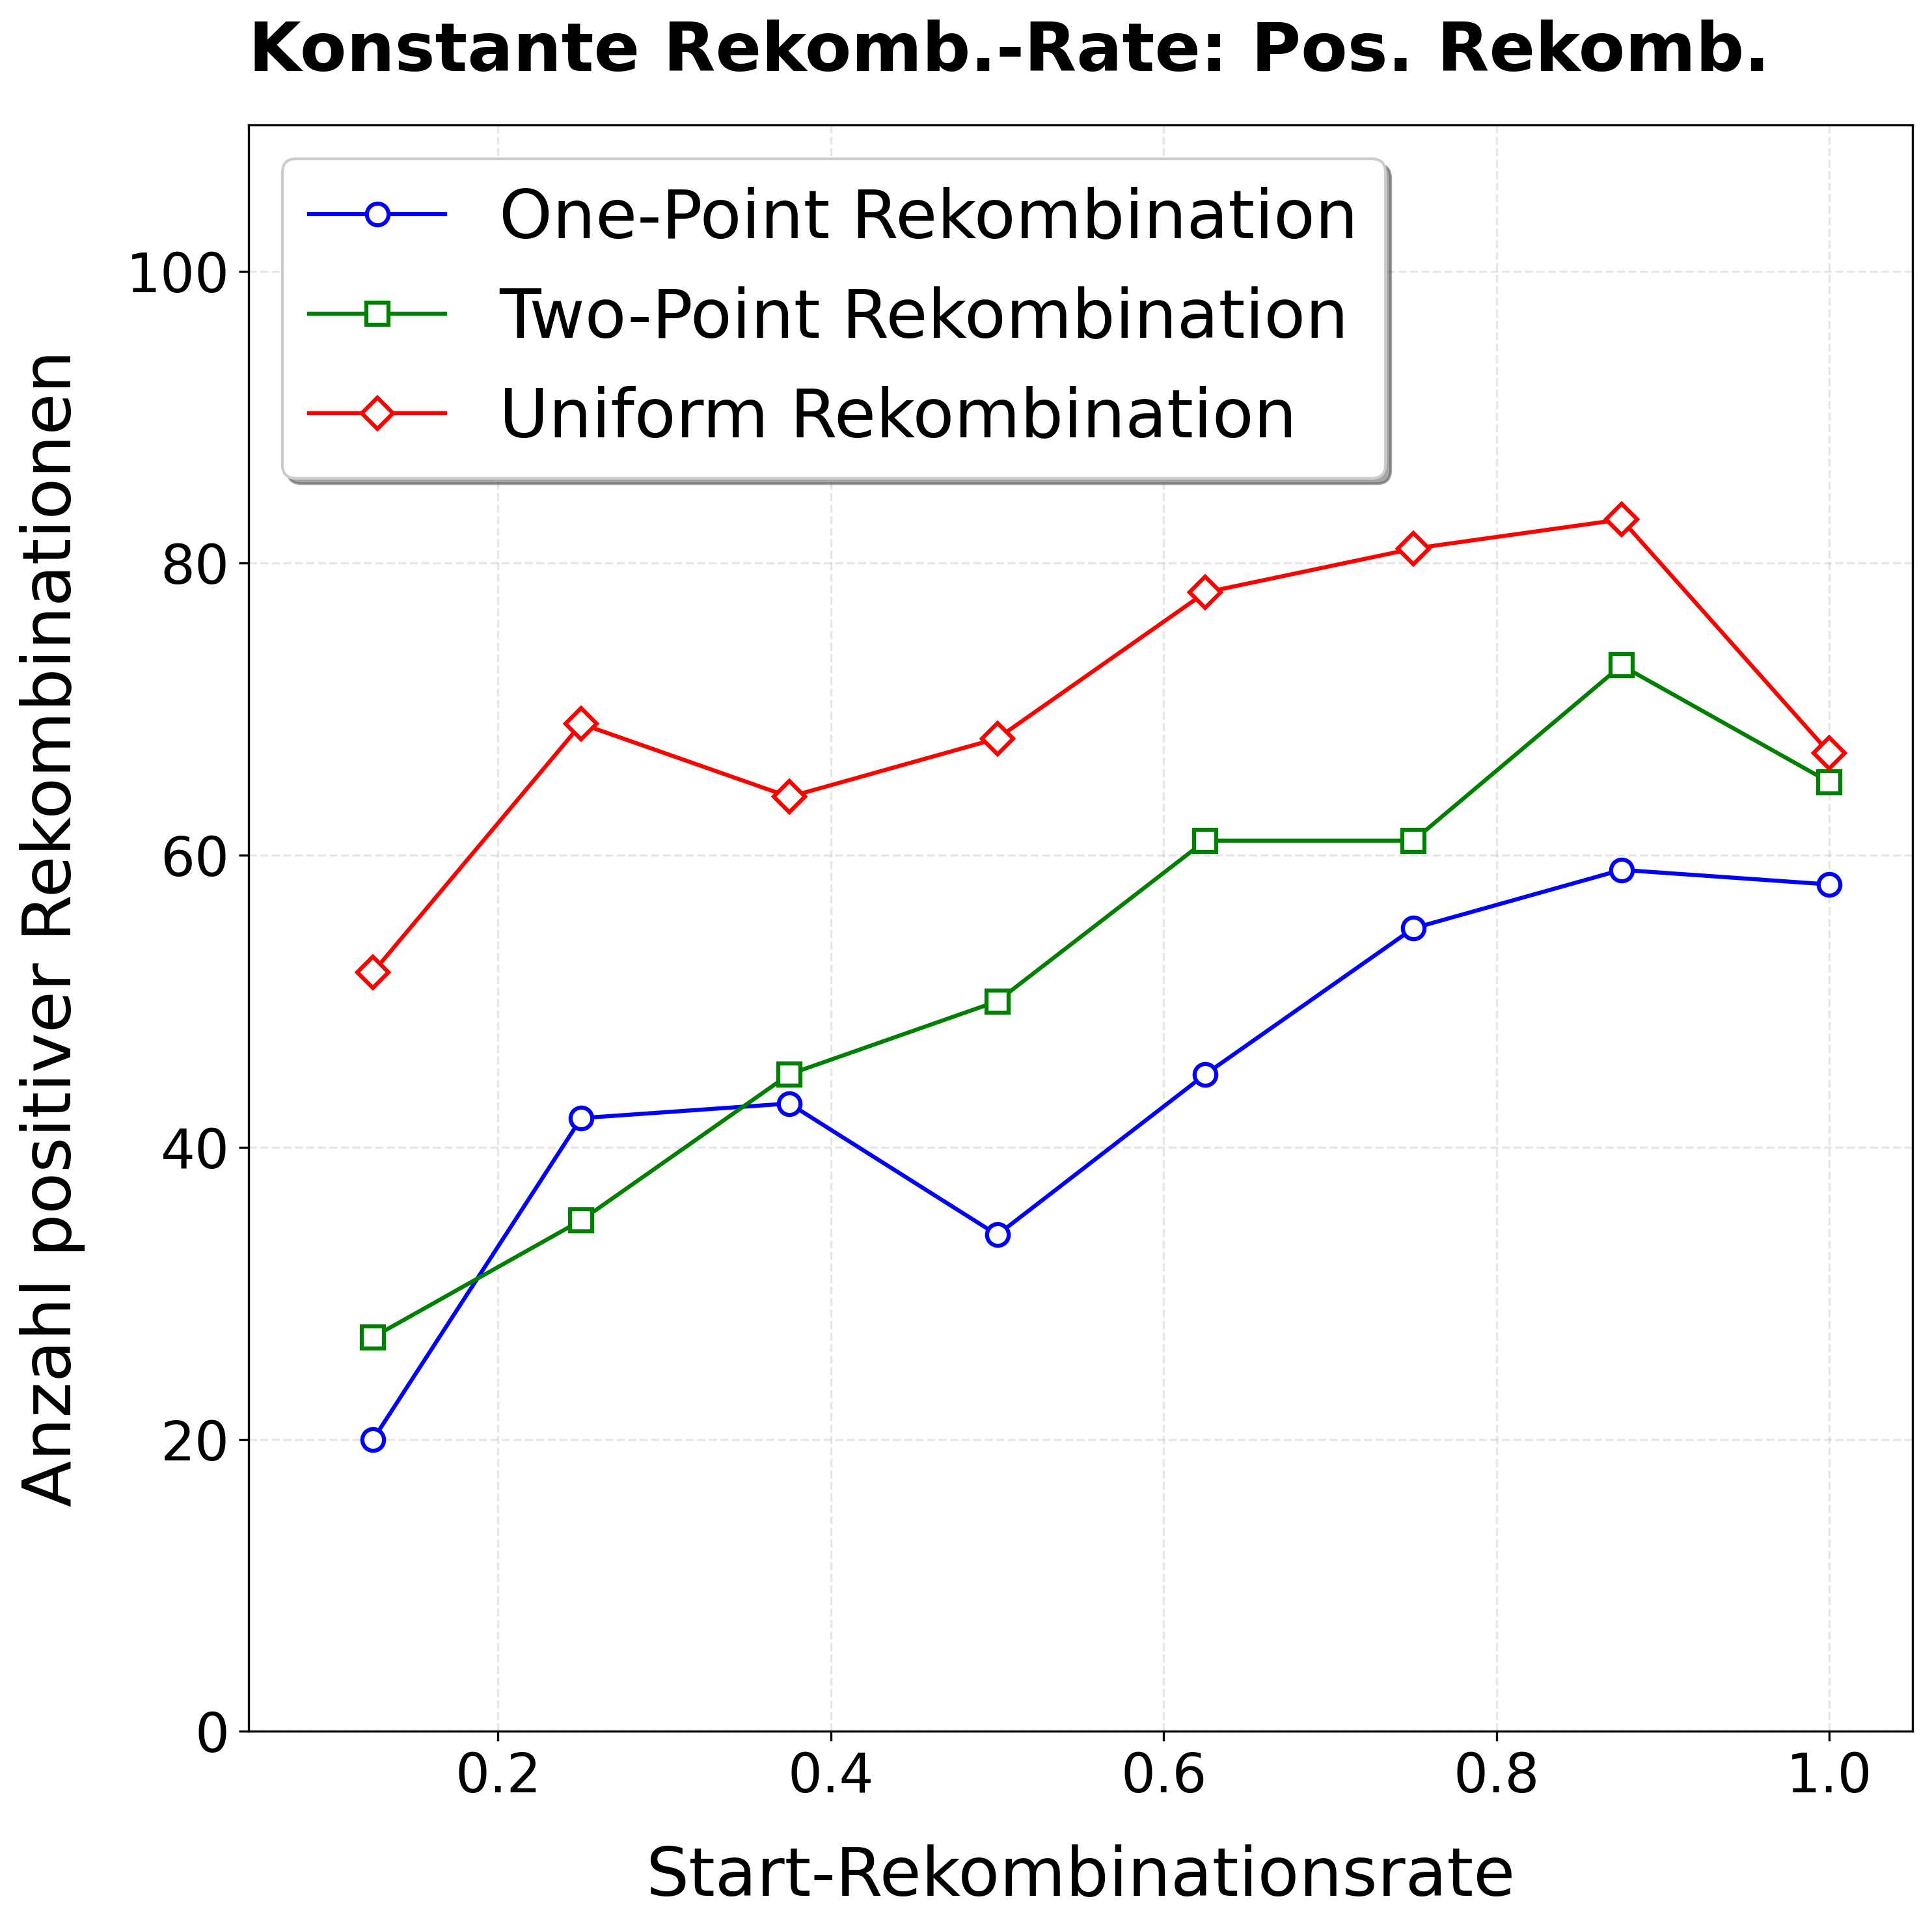
\includegraphics[width=\textwidth]{Bilder/EncodePlotPositiveRekombinationKonstant.png}
		\caption{Konstant}
		\label{fig:encodePosRekombinationKonstant}
	\end{subfigure}%
	\hfill
	\begin{subfigure}[b]{0.32\textwidth}
		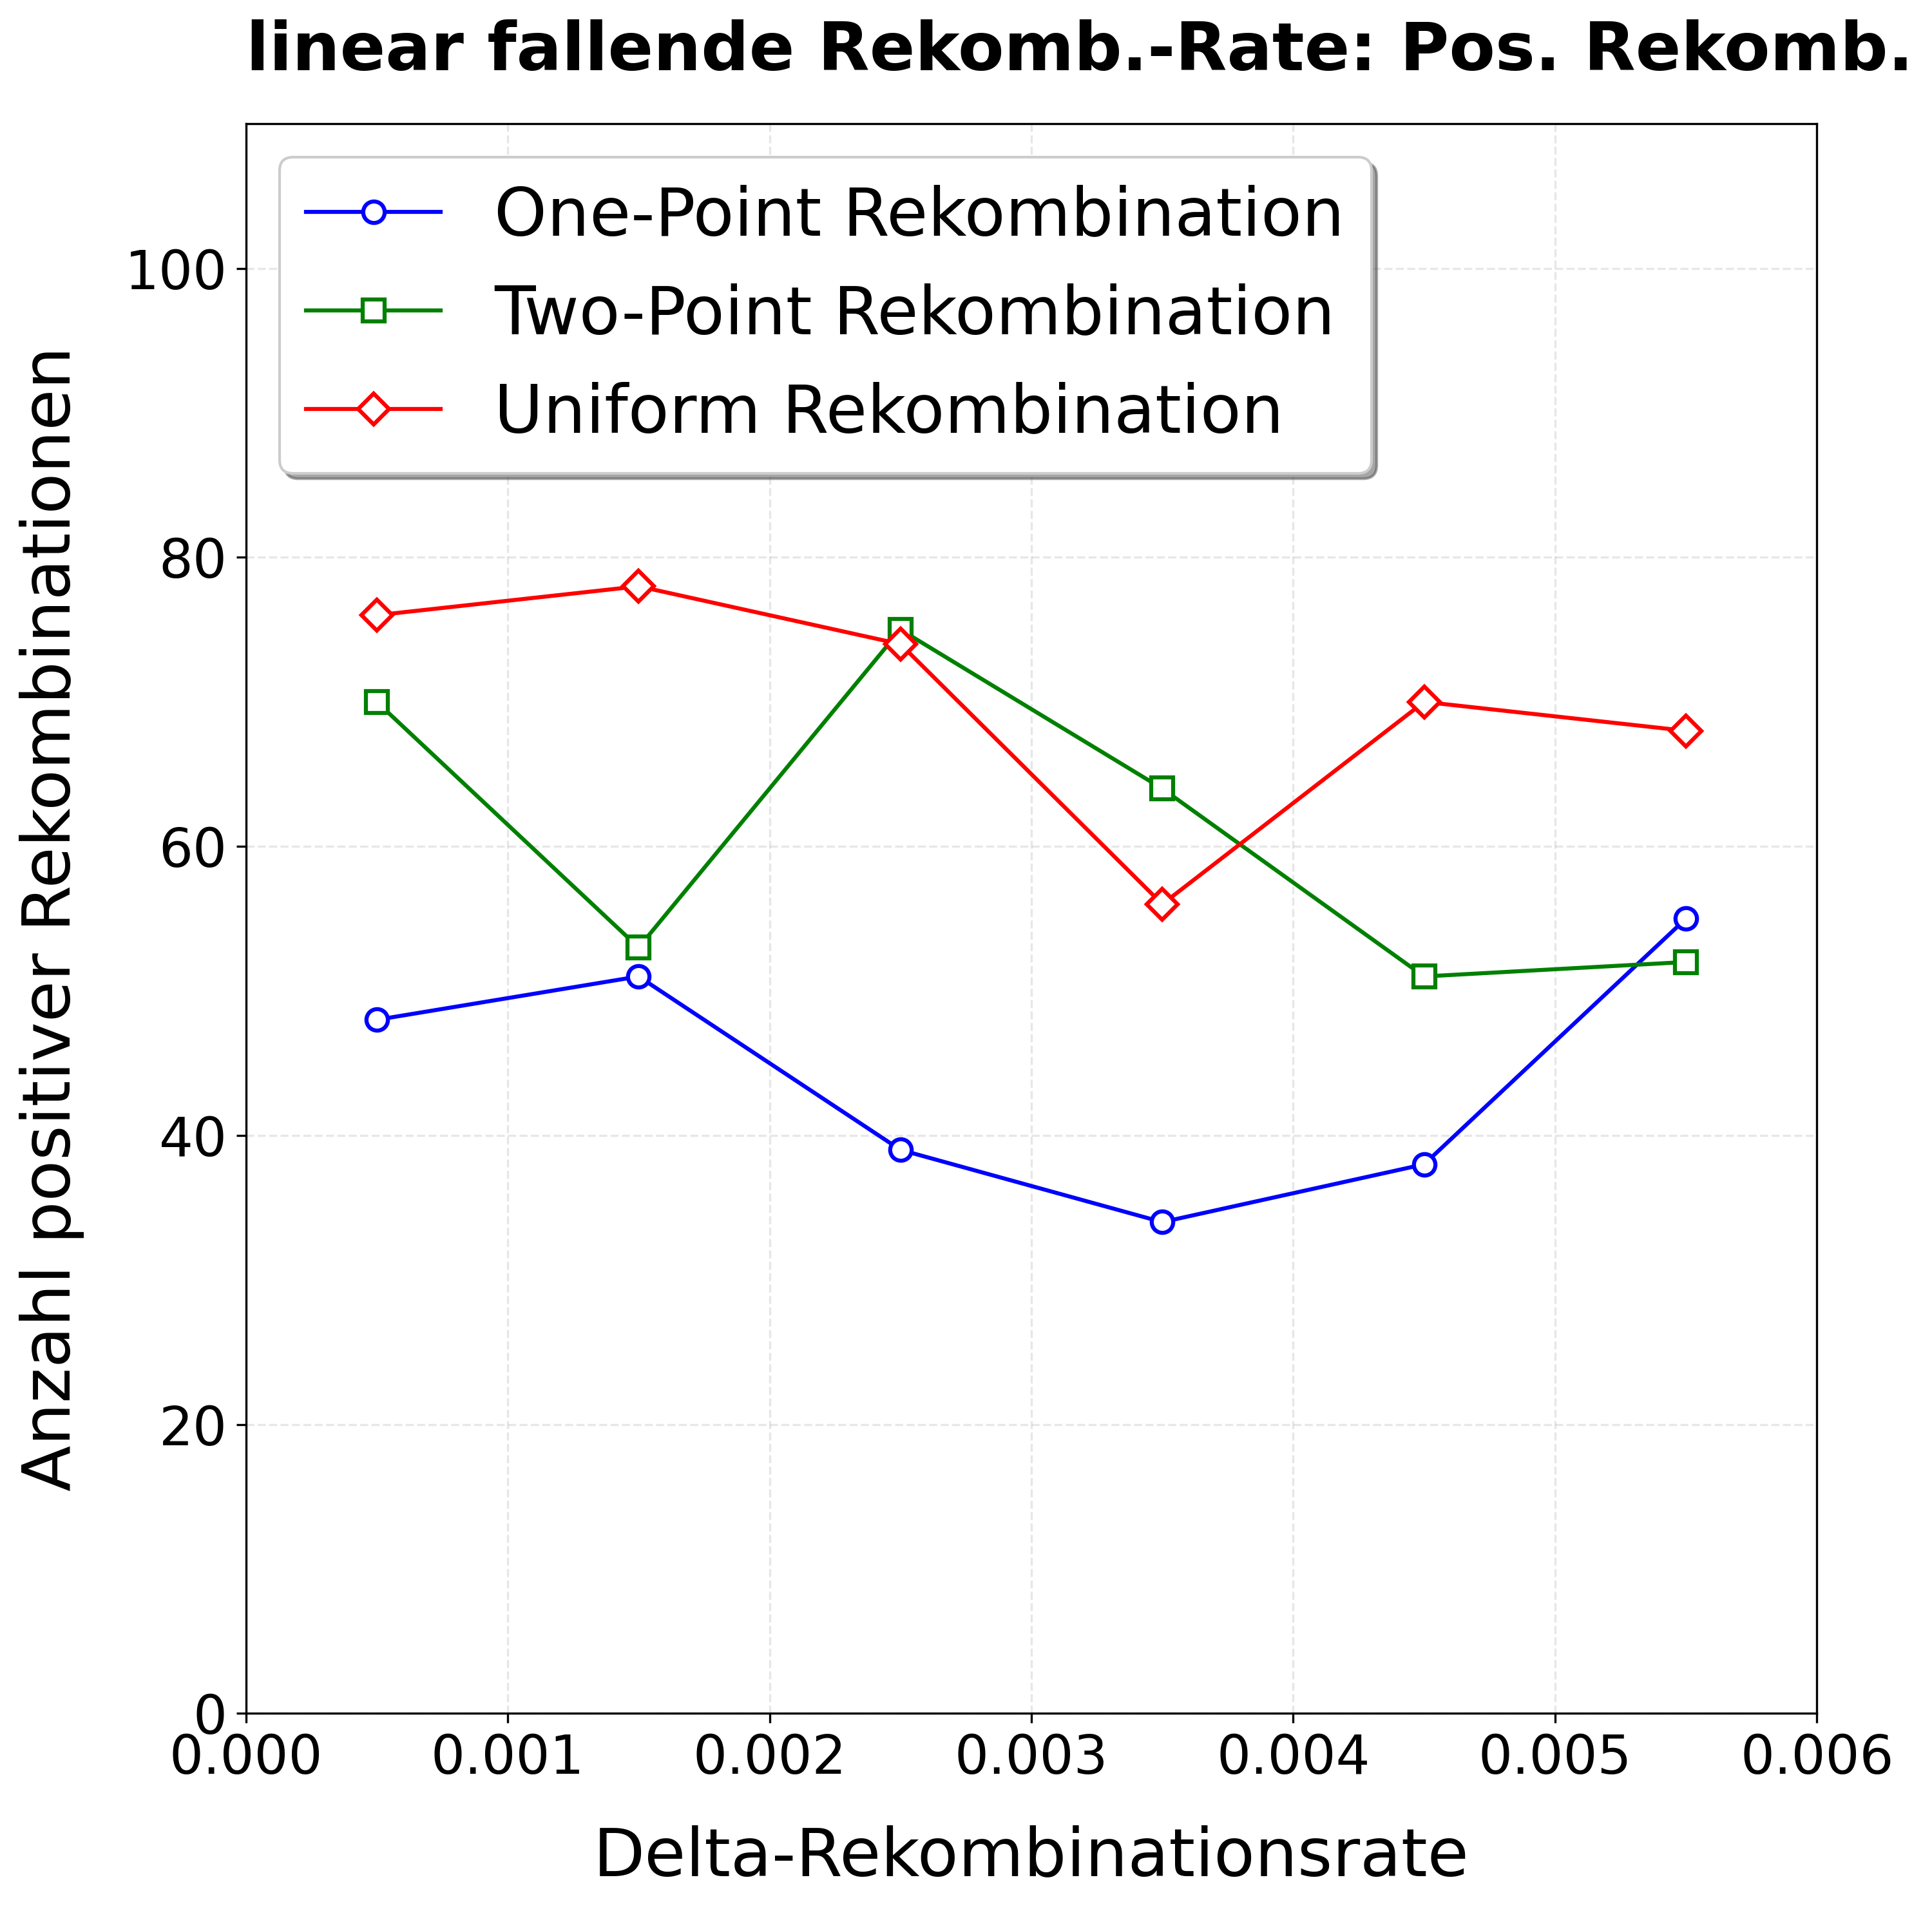
\includegraphics[width=\textwidth]{Bilder/EncodePlotPositiveRekombinationClegg.png}
		\caption{linear fallend}
		\label{fig:encodePosRekombinationClegg}
	\end{subfigure}%
	\hfill
	\begin{subfigure}[b]{0.32\textwidth}
		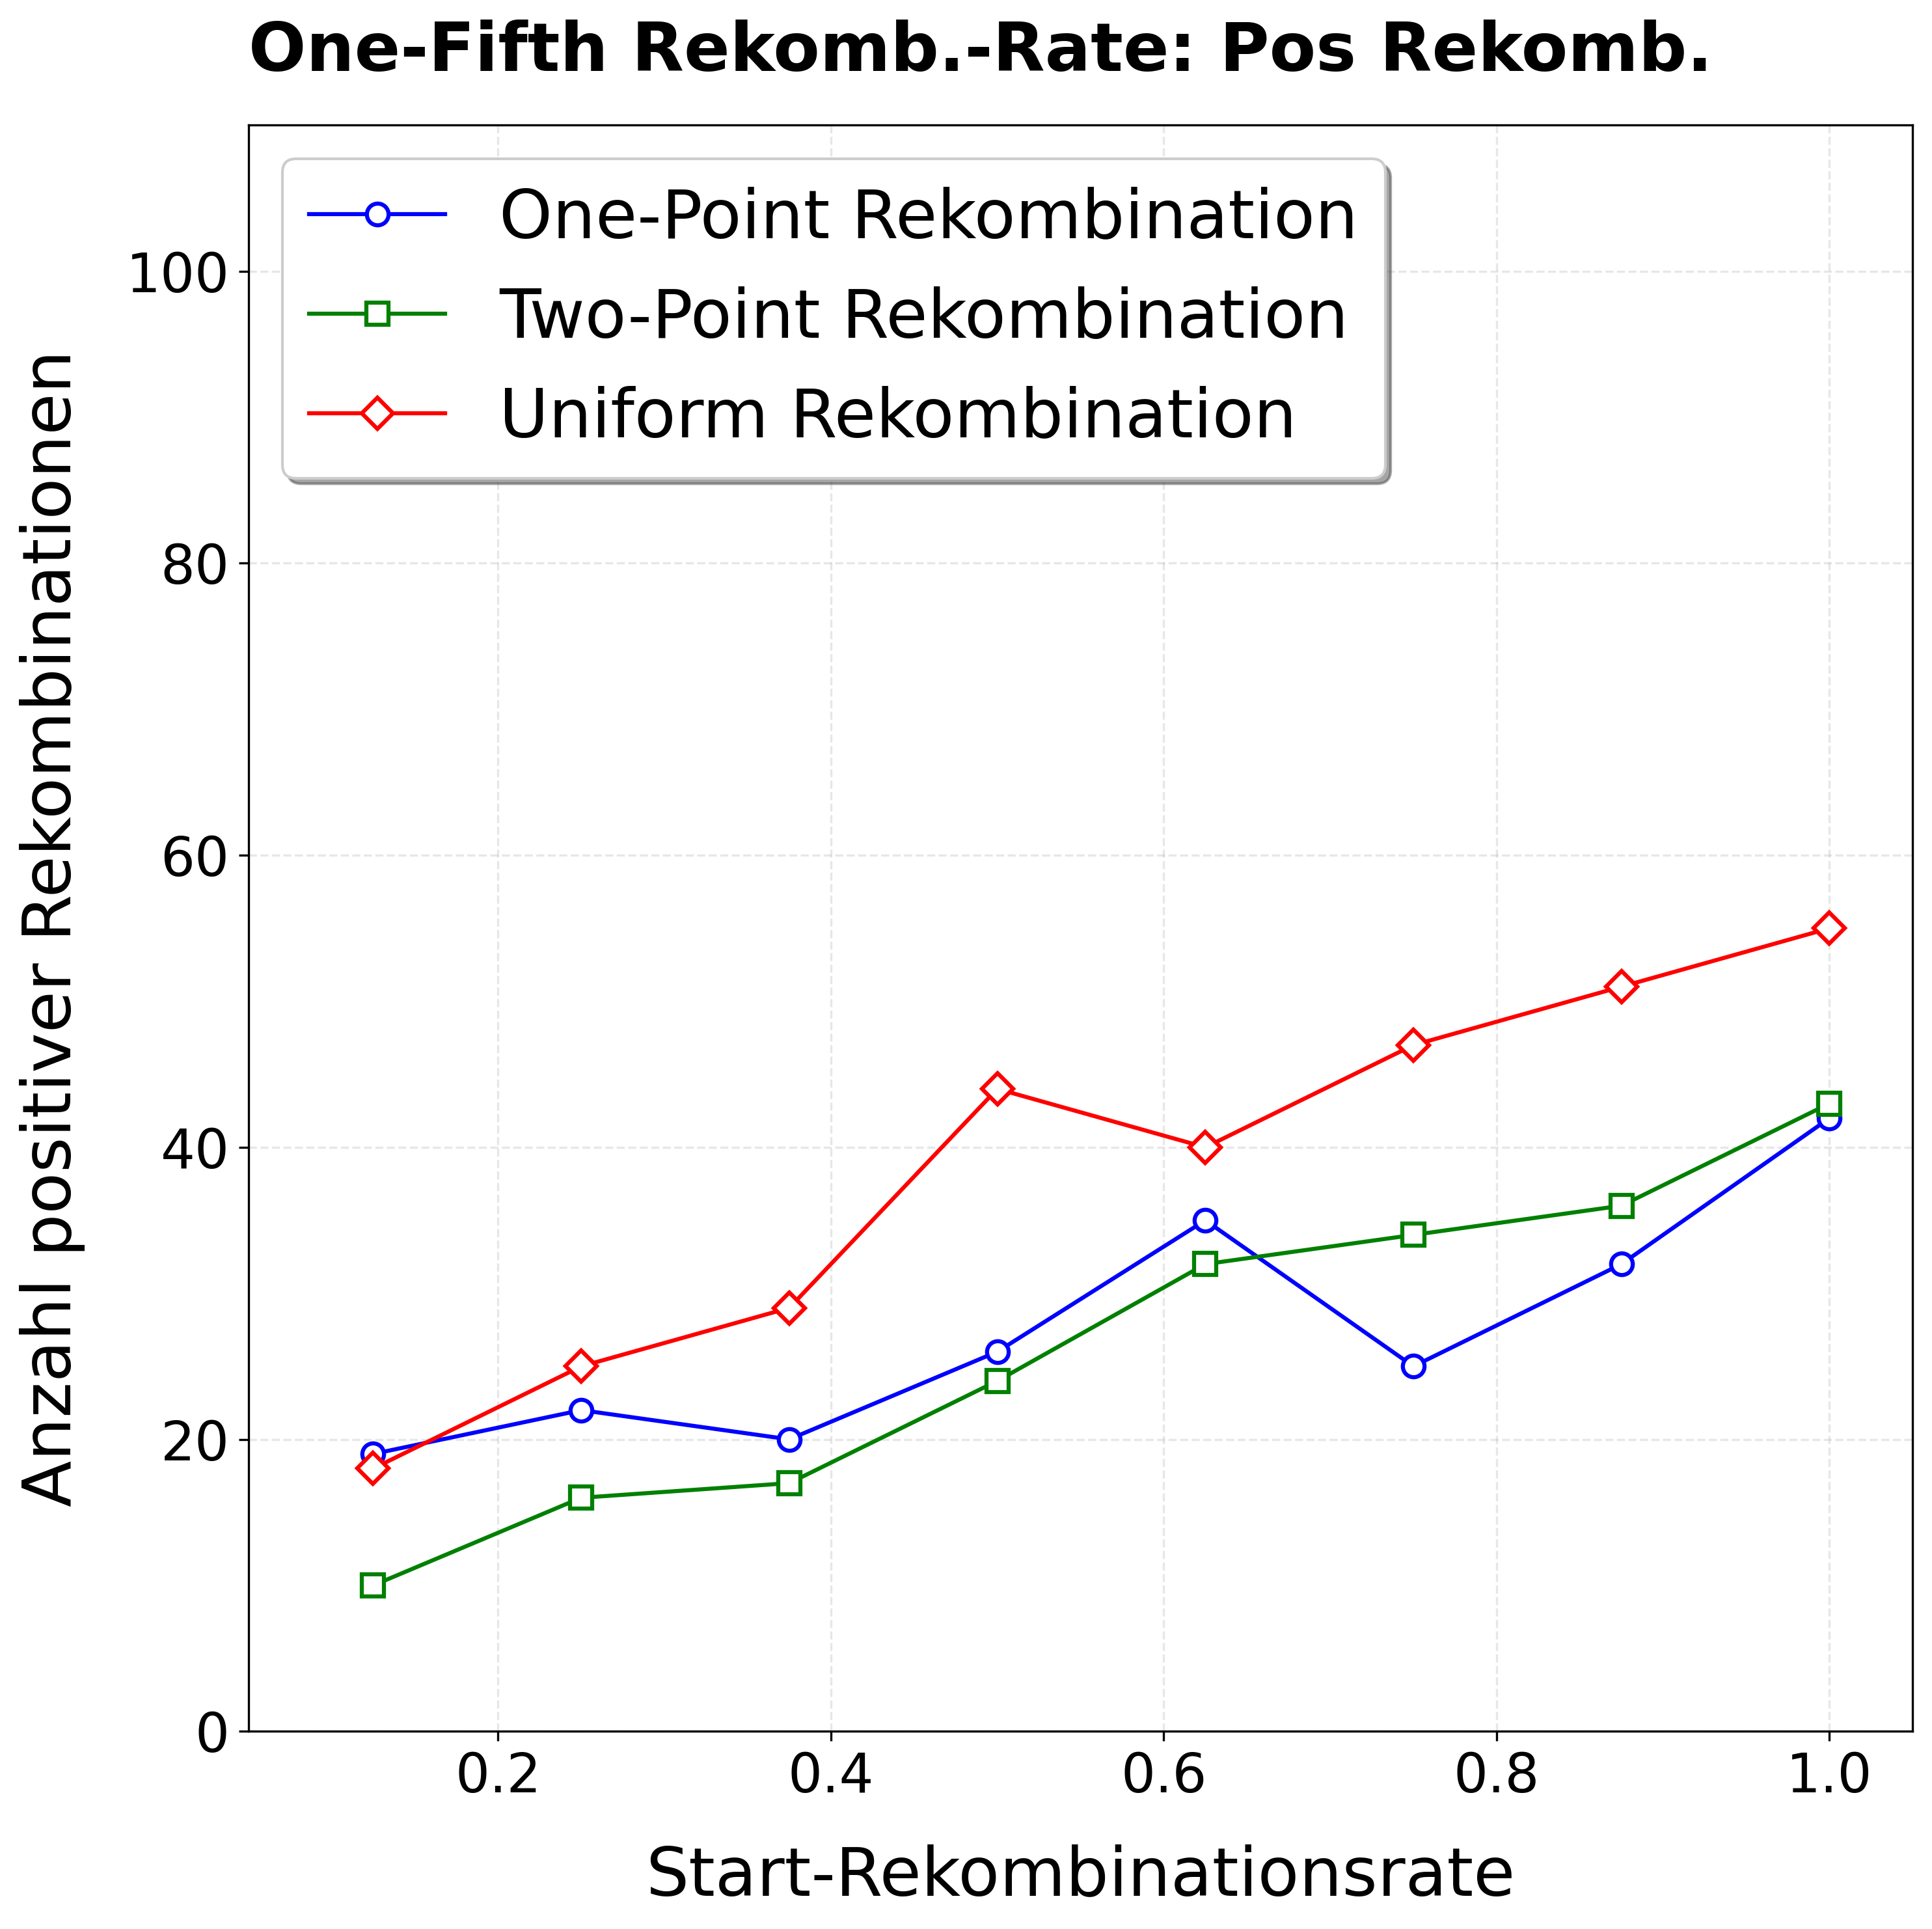
\includegraphics[width=\textwidth]{Bilder/EncodePlotPositiveRekombinationOneFifth.png}
		\caption{One-Fifth Regel}
		\label{fig:encodePosRekombinationOneFifth}
	\end{subfigure}
	\caption{Encode: Raten-Arten und Anzahl positive Rekombinationen}
	\label{fig:encodePosRekombination}
\end{figure}

In Abbildung \ref{fig:encodePosRekombination} kann beobachtet werden, dass für jede Rekombinationsraten-Art die Uniform Rekombination die höchsten Anzahlen an positiver Rekombination produziert.
Für die konstante und linear fallende Rekombinationsrate ist die Two-Point Rekombination in dieser Hinsicht besser als die One-Point Rekombination.
Auch wird ersichtlich, dass die Rekombinationsrate mit der One-Fifth Regel niedrigere Rekombinationserfolge einfährt als die anderen Rekombinationsraten-Arten.\\
Eine höhere Rekombinationsrate bedeutet auch eine höhere Chance, dass die Rekombination ausgeführt wird und somit die Fitness verbessert.
So ist es nicht überraschend, dass die Abbildungen \ref{fig:encodePosRekombinationKonstant} und \ref{fig:encodePosRekombinationOneFifth} insgesamt eine positive Steigung aufzeigen.
Nicht ersichtlich ist allerdings, wieso die konstanten Rekombinationsraten gleich 1,0 weniger gute Ergebnisse liefern als die konstanten Rekombinationsraten gleich 0,875.
Dies gilt für alle Rekombinationsarten mit der konstanten Rekombinationsrate.\\
Ebenfalls überraschend sind die kurzfristigen lokalen Maxima, die die Abbildungen \ref{fig:encodePosRekombinationKonstant} und \ref{fig:encodePosRekombinationOneFifth} bei geringen Rekombinationsraten aufzeigen.
Die hohen Anzahlen an positiven Rekombinationen, obwohl die Rekombination nicht wahrscheinlich ausgeführt wird, könnte darauf hindeuten, dass die ausgeführten Rekombinationsschritte effektiver waren als diejenigen Rekombinationsschritte, die häufiger ausgeführt werden.


\subsection{Rohdatenanalyse: Koza}
\label{subsec:rohdatenKoza}

Die folgenden Tabellen \ref{table:kozaOnePointRohdaten}, \ref{table:kozaTwoPointRohdaten} und \ref{table:kozaUniformRohdaten} zeigen die Rohdaten-Auswertungen des Koza-Testszenarios.
Für jede CGP-Konfiguration wurden 50 Modelle innerhalb von maximal 50000 Iterationen trainiert.
Jede der Tabellen stellt eine Rekombinationsart mit verschiedenen Parametrierungen der Rekombinationsraten dar.
Wie in Abschnitt \ref{subsec:rohdatenEncode} wurde für das Koza-Testszenario der Offset als Parameter ausgestellt.
Dies geht aus den Ergebnissen von Parity und Keijzer hervor, bei denen keine erfolgreichen Rekombinationsschritte ausgeführt wurden, wenn ein Offset aktiv war.
Da mit dieser Arbeit die Effizienz der Rekombination ausgewertet werden soll, ist es sinnvoll den Offset nicht näher zu betrachten, um den vollen Umfang der Fitnessverbesserungen durch Rekombination zu bewerten.
Ziel des Abschnittes ist es die Zusammenhänge zwischen verschiedenen Rekombinationsraten-Arten und dem Erfolg des CGP-Trainings zu finden.
Außerdem soll bestimmt werden, welche Metrik für die Auswertung der bayes'schen Analyse verwendet werden soll.
In diesem Abschnitt werden nur die Ergebnisse von Koza ausgewertet und erlauben noch keine allgemeinen Aussagen.
Diese werden in Abschnitt \ref{subsec:rohdatenZusammenfassung} ausgewertet, indem die Ergebnisse aus allen Testszenarien zusammengetragen und verglichen werden.


\begin{table}[H]
	\centering
	\begin{tabular}{c | c | c | c | c | c | c}
		\begin{turn}{270} \textbf{CGP-Konfigurationen} \end{turn} & \begin{turn}{270} \textbf{Anzahl pos. Mutationen} \end{turn} & \begin{turn}{270} \textbf{Anzahl pos. Rekomb.} \end{turn} & \begin{turn}{270} \textbf{Anzahl neg. Mutationen} \end{turn} & \begin{turn}{270} \textbf{Median Iter. pos. Rekomb.} \end{turn} & \begin{turn}{270} \textbf{Median Iter. bis Konv.} \end{turn} & \begin{turn}{270} \textbf{Stopp-Kriterium erfüllt} \end{turn}\\
		\hline
		keine Rekombination & 1157 & - & - & - & 208 & 48\\
		\hline
		One-Point Konstant: 0,125 & 1338 & 9 & 8 & 42 & 616 & 41\\
		\hline
		One-Point Konstant: 0,25 & 1180 & 23 & 16 & 7 & 611 & 45\\
		\hline
		One-Point Konstant: 0,375 & 1493 & 42 & 25 & 43 & 2012 & 47\\
		\hline
		One-Point Konstant: 0,5 & 1477 & 57 & 40 & 18 & 602,5 & 36\\
		\hline
		One-Point Konstant: 0,625 & 1287 & 48 & 23 & 82,5 & 2302 & 45\\
		\hline
		One-Point Konstant: 0,75 & 1423 & 65 & 43 & 29 & 989 & 47\\
		\hline
		One-Point Konstant: 0,875 & 1593 & 85 & 48 & 18 & 848 & 34\\
		\hline
		One-Point Konstant: 1,0 & 1548 & 136 & 83 & 73,5 & 667 & 41\\
		\hline
		One-Point Clegg: 0,0005 & 1460 & 98 & 56 & 45,5 & 603 & 43\\
		\hline
		One-Point Clegg: 0,0015 & 1525 & 78 & 43 & 12 & 659 & 40\\
		\hline
		One-Point Clegg: 0,0025 & 1303 & 52 & 31 & 7 & 583 & 41\\
		\hline
		One-Point Clegg: 0,0035 & 1233 & 61 & 35 & 6 & 529 & 42\\
		\hline
		One-Point Clegg: 0,0045 & 1187 & 62 & 36 & 10 & 511 & 44\\
		\hline
		One-Point Clegg: 0,0055 & 1622 & 50 & 28 & 9,5 & 1320 & 42\\
		\hline
		One-Point One-Fifth: 0,125 & 1434 & 2 & 1 & 1,5 & 462 & 44\\
		\hline
		One-Point One-Fifth: 0,25 & 1544 & 7 & 6 & 1 & 1400 & 44\\
		\hline
		One-Point One-Fifth: 0,375 & 1005 & 13 & 8 & 2 & 838,5 & 46\\
		\hline
		One-Point One-Fifth: 0,5 & 1137 & 14 & 10 & 2 & 360,5 & 41\\
		\hline
		One-Point One-Fifth: 0,625 & 1207 & 18 & 12 & 2 & 947 & 44\\
		\hline
		One-Point One-Fifth: 0,75 & 1387 & 17 & 11 & 3 & 910 & 43\\
		\hline
		One-Point One-Fifth: 0,875 & 1160 & 29 & 14 & 4 & 301 & 43\\
		\hline
		One-Point One-Fifth: 1,0 & 1393 & 38 & 25 & 4 & 568 & 43\\
	\end{tabular}
	\caption{Koza One-Point Rekombination: Auswertung der Rohdaten}
	\label{table:kozaOnePointRohdaten}
\end{table}



\begin{table}[H]
	\centering
	\begin{tabular}{c | c | c | c | c | c | c}
		\begin{turn}{270} \textbf{CGP-Konfigurationen} \end{turn} & \begin{turn}{270} \textbf{Anzahl pos. Mutationen} \end{turn} & \begin{turn}{270} \textbf{Anzahl pos. Rekomb.} \end{turn} & \begin{turn}{270} \textbf{Anzahl neg. Mutationen} \end{turn} & \begin{turn}{270} \textbf{Median Iter. pos. Rekomb.} \end{turn} & \begin{turn}{270} \textbf{Median Iter. bis Konv.} \end{turn} & \begin{turn}{270} \textbf{Stopp-Kriterium erfüllt} \end{turn}\\
		\hline
		keine Rekombination & 1157 & - & - & - & 208 & 48\\
		\hline
		Two-Point Konstant: 0,125 & 1383 & 41 & 24 & 106 & 106 & 45\\
		\hline
		Two-Point Konstant: 0,25 & 1475 & 82 & 55 & 47,5 & 613 & 48\\
		\hline
		Two-Point Konstant: 0,375 & 1207 & 91 & 58 & 75 & 153 & 43\\
		\hline
		Two-Point Konstant: 0,5 & 1120 & 85 & 49 & 29 & 194 & 46\\
		\hline
		Two-Point Konstant: 0,625 & 1013 & 93 & 38 & 16 & 124 & 49\\
		\hline
		Two-Point Konstant: 0,75 & 1373 & 145 & 65 & 21 & 190 & 43\\
		\hline
		Two-Point Konstant: 0,875 & 1400 & 140 & 76 & 26 & 731 & 46\\
		\hline
		Two-Point Konstant: 1,0 & 1176 & 220 & 140 & 50,5 & 207 & 48\\
		\hline
		Two-Point Clegg: 0,0005 & 1446 & 193 & 99 & 30 & 205 & 47\\
		\hline
		Two-Point Clegg: 0,0015 & 1167 & 105 & 59 & 14 & 154 & 45\\
		\hline
		Two-Point Clegg: 0,0025 & 1396 & 106 & 53 & 18 & 504,5 & 44\\
		\hline
		Two-Point Clegg: 0,0035 & 1043 & 95 & 45 & 13 & 142 & 46\\
		\hline
		Two-Point Clegg: 0,0045 & 1023 & 100 & 50 & 14,5 & 96 & 46\\
		\hline
		Two-Point Clegg: 0,0055 & 1160 & 94 & 43 & 11,5 & 223,5 & 49\\
		\hline
		Two-Point One-Fifth: 0,125 & 1422 & 5 & 4 & 2 & 226 & 45\\
		\hline
		Two-Point One-Fifth: 0,25 & 1348 & 10 & 5 & 4 & 404,5 & 44\\
		\hline
		Two-Point One-Fifth: 0,375 & 1365 & 15 & 4 & 3 & 460 & 46\\
		\hline
		Two-Point One-Fifth: 0,5 & 1761 & 15 & 4 & 5 & 584 & 47\\
		\hline
		Two-Point One-Fifth: 0,625 & 1165 & 22 & 13 & 6 & 165 & 48\\
		\hline
		Two-Point One-Fifth: 0,75 & 1041 & 26 & 13 & 4 & 213,5 & 46\\
		\hline
		Two-Point One-Fifth: 0,875 & 1050 & 42 & 19 & 7 & 185 & 48\\
		\hline
		Two-Point One-Fifth: 1,0 & 1142 & 35 & 20 & 5 & 348 & 49\\
	\end{tabular}
	\caption{Koza Two-Point Rekombination: Auswertung der Rohdaten}
	\label{table:kozaTwoPointRohdaten}
\end{table}




\begin{table}[H]
	\centering
	\begin{tabular}{c | c | c | c | c | c | c}
		\begin{turn}{270} \textbf{CGP-Konfigurationen} \end{turn} & \begin{turn}{270} \textbf{Anzahl pos. Mutationen} \end{turn} & \begin{turn}{270} \textbf{Anzahl pos. Rekomb.} \end{turn} & \begin{turn}{270} \textbf{Anzahl neg. Mutationen} \end{turn} & \begin{turn}{270} \textbf{Median Iter. pos. Rekomb.} \end{turn} & \begin{turn}{270} \textbf{Median Iter. bis Konv.} \end{turn} & \begin{turn}{270} \textbf{Stopp-Kriterium erfüllt} \end{turn}\\
		\hline
		keine Rekombination & 1157 & - & - & - & 208 & 48\\
		\hline
		Uniform Konstant: 0,125 & 1178 & 124 & 75 & 31,5 & 316 & 44\\
		\hline
		Uniform Konstant: 0,25 & 1233 & 157 & 90 & 44 & 479 & 43\\
		\hline
		Uniform Konstant: 0,375 & 1166 & 251 & 132 & 35 & 257,5 & 47\\
		\hline
		Uniform Konstant: 0,5 & 1084 & 184 & 92 & 27,5 & 113 & 45\\
		\hline
		Uniform Konstant: 0,625 & 1277 & 295 & 152 & 31 & 430 & 47\\
		\hline
		Uniform Konstant: 0,75 & 1301 & 276 & 141 & 31 & 382 & 43\\
		\hline
		Uniform Konstant: 0,875 & 1102 & 332 & 181 & 31 & 467 & 44\\
		\hline
		Uniform Konstant: 1,0 & 1080 & 328 & 199 & 21 & 176 & 43\\
		\hline
		Uniform Clegg: 0,0005 & 1155 & 373 & 197 & 40 & 709 & 46\\
		\hline
		Uniform Clegg: 0,0015 & 793 & 259 & 147 & 17 & 81 & 48\\
		\hline
		Uniform Clegg: 0,0025 & 887 & 319 & 181 & 25 & 140 & 48\\
		\hline
		Uniform Clegg: 0,0035 & 1415 & 318 & 162 & 18 & 162 & 46\\
		\hline
		Uniform Clegg: 0,0045 & 1404 & 304 & 153 & 18 & 637 & 48\\
		\hline
		Uniform Clegg: 0,0055 & 1364 & 300 & 141 & 19 & 143 & 46\\
		\hline
		Uniform One-Fifth: 0,125 & 1545 & 12 & 6 & 5 & 147 & 41\\
		\hline
		Uniform One-Fifth: 0,25 & 1314 & 24 & 8 & 6 & 153 & 44\\
		\hline
		Uniform One-Fifth: 0,375 & 1384 & 36 & 14 & 8,5 & 273 & 47\\
		\hline
		Uniform One-Fifth: 0,5 & 1718 & 61 & 28 & 6 & 848 & 46\\
		\hline
		Uniform One-Fifth: 0,625 & 1244 & 72 & 35 & 6 & 363 & 47\\
		\hline
		Uniform One-Fifth: 0,75 & 1320 & 90 & 49 & 5 & 207 & 44\\
		\hline
		Uniform One-Fifth: 0,875 & 1406 & 92 & 49 & 9 & 470 & 46\\
		\hline
		Uniform One-Fifth: 1,0 & 1444 & 83 & 40 & 6 & 794,5 & 47\\
	\end{tabular}
	\caption{Koza Uniform Rekombination: Auswertung der Rohdaten}
	\label{table:kozaUniformRohdaten}
\end{table}

Aus den Spalten \glqq Stopp-Kriterium erfüllt\grqq\space der drei Tabellen \ref{table:kozaOnePointRohdaten}, \ref{table:kozaTwoPointRohdaten} und \ref{table:kozaUniformRohdaten} geht hervor, dass relativ viele Durchgänge des CGP-Trainings konvergiert sind.
Deswegen wird für die bayes'sche Analyse in Abschnitt \ref{subsec:bayesKoza} die Anzahl an Iterationen bis zur Konvergenz als Metrik verwendet.
Außerdem lässt sich erkennen, dass mehr Mutationen zu einer Verbesserung der Fitness geführt haben als es die Rekombinationsschritte getan haben.
Gleichzeitig werden einige Erfolge der Rekombinationsschritte verloren, indem anschließend noch eine Mutation ausgeführt wurde, wie in den Spalten \glqq Anzahl negative Mutationen\grqq\space zu sehen ist.
Dies kann dadurch passieren, dass die Auswahl der Elitisten erst nach der Mutation getroffen wird und so keine Evaluation der Fitness zwischen Rekombination und Mutation stattfindet.
Eine Möglichkeit dies zu beheben wäre es, die Elitisten nach der Rekombination mit den Elitisten nach der Mutation abzugleichen und so die besten Chromosomen zu verwenden, die aus beiden genetischen Operationen resultieren.\\
Die Rekombination ist dabei vor allem in den frühen Iterationen erfolgreich.
Dabei unterscheiden sich die unterschiedlichen Rekombinationsraten-Arten.
Die Rekombination mit der One-Fifth Regel weist vor allem in den ersten Iterationen Erfolge auf, mit der linear fallenden Rekombinationsrate ist der Median etwas höher und mit der konstanten Rekombinationsrate sind teilweise relativ hohe Iterationen noch erfolgreich.
Für die konstante Rekombinationsrate werden diese hohen Iterationsmediane allerdings nur für die One-Point und Two-Point Rekombination gesichtet.
Dabei fällt auf, dass diese späten Rekombinationserfolge im Training nicht im Zusammenhang mit der Höhe der Rekombinationsrate stehen, da einige erhöhte Werte in den Spalten \glqq Median Iterationen positive Rekombination\grqq\space auch für kleinere Rekombinationsraten auftauchen.
Außerdem kann kein Zusammenhang zwischen den Spalten \glqq Median Iterationen positive Rekombination\grqq\space und \glqq Median Iterationen bis Konvergenz\grqq\space gefunden werden.
Das bedeutet, dass die Rekombinationserfolge nicht durch längeres Training automatisch auch zu späteren Iterationen stattfinden, sondern dass dieses Verhalten unabhängig von der Trainingsdauer auftritt.
Dieses Wissen könnte genutzt werden, um so Rekombination gezielter einzusetzen.
Beispielsweise könnte man die frühen Rekombinationserfolge der linear fallenden Rekombinationsrate nutzen, wobei diese ähnlich viele positive Rekombinationen aufweist wie die konstante Rekombinationsrate.
So könnte man in den ersten Iterationen die Erfolge der Rekombination nutzen und anschließend die Rekombinationsrate schneller reduzieren.\\
Werden die Iterationen betrachtet, die die Modelle bis zur Konvergenz gebraucht haben, lässt sich feststellen, dass die CGP-Modelle mit Two-Point Rekombination durchschnittlich weniger Iterationen (278) gebraucht hat als die anderen.
Darauf folgt die Uniform Rekombination (349 Iterationen) und anschließend die One-Point Rekombination (835 Iterationen).
Demnach sind alle Mittelwerte der Iterationsmediane bis zur Konvergenz größer als der Median der Anzahl an Iterationen, die das CGP-Modell ohne Rekombination gebraucht hat (208).
Dabei muss allerdings beachtet werden, dass bei der CGP-Konfiguration ohne Rekombination alle Hyperparameter optimiert wurden.
Demnach liefern die CGP-Modelle ohne Rekombination optimierte Ergebnisse während alle anderen CGP-Konfigurationen dieses Potential noch ausschöpfen können.
Trotzdem können für einige vereinzelte CGP-Konfigurationen bereits frühere Konvergenzen bei gleicher Anzahl an erfüllten Stopp-Kriterien beobachtet werden.
Ein Beispiel bietet die Konfiguration \glqq Uniform Clegg: 0,0015\grqq\space aus Tabelle \ref{table:kozaUniformRohdaten}.
Dies ist ein Anzeichen dafür, dass CGP-Modelle durch Rekombination effizienter werden können, wenn die Rekombination sinnvoll eingesetzt wird.\\
Des weiteren wurde beim Vergleich der Spalten \glqq Anzahl positive Rekombinationen\grqq, \glqq Anzahl negative Mutationen\grqq\space und \glqq Median Iterationen positive Rekombinationen\grqq mit den Spalten \glqq Median Iterationen bis Konvergenz\grqq\space und \glqq Stopp-Kriterium erfüllt\grqq\space keine zusammenhängenden Muster erkannt.
Eine Möglichkeit dafür, dass die Anzahl der positiven Rekombinationen keine deutliche Veränderungen in der Effizienz des CGPs hervorruft, könnten die negativen Mutationen sein.
In weiteren Tests könnte dieser Zusammenhang untersucht werden, indem keine Mutation ausgeführt wird, wenn bereits eine Rekombination die Fitness des Modells verbessert hat.
So könnte überprüft werden, ob die CGP-Modelle mit mehr Rekombinationserfolgen auch bessere Ergebnisse liefern oder ob Mutationserfolge relevanter für ein erfolgreiches CGP-Training sind.\\
Ein weiterer Punkt der auffällt sind die relativ hohen Zahlen der negativen Mutationen im Koza-Testszenario.
Dies könnte daran liegen, dass die Fitness-Werte in SR Benchmarks kontinuierlich sind, während sie in booleschen Problemen durch diskrete Werte abgebildet werden.
Dadurch können auch kleinere Trainingserfolge durch Rekombination in den Tabellen abgebildet werden.
Dies könnte bedeuten, dass vor allen bei SR die Evaluierung nach der Rekombination als Zwischenschritt sinnvoll sein könnte.\\
Um die positiven Rekombinationen zu bewerten wird folgende Abbildung \ref{fig:kozaPosRekombination} eingeführt:

\begin{figure}[H]
	\centering
	\begin{subfigure}[b]{0.32\textwidth}
		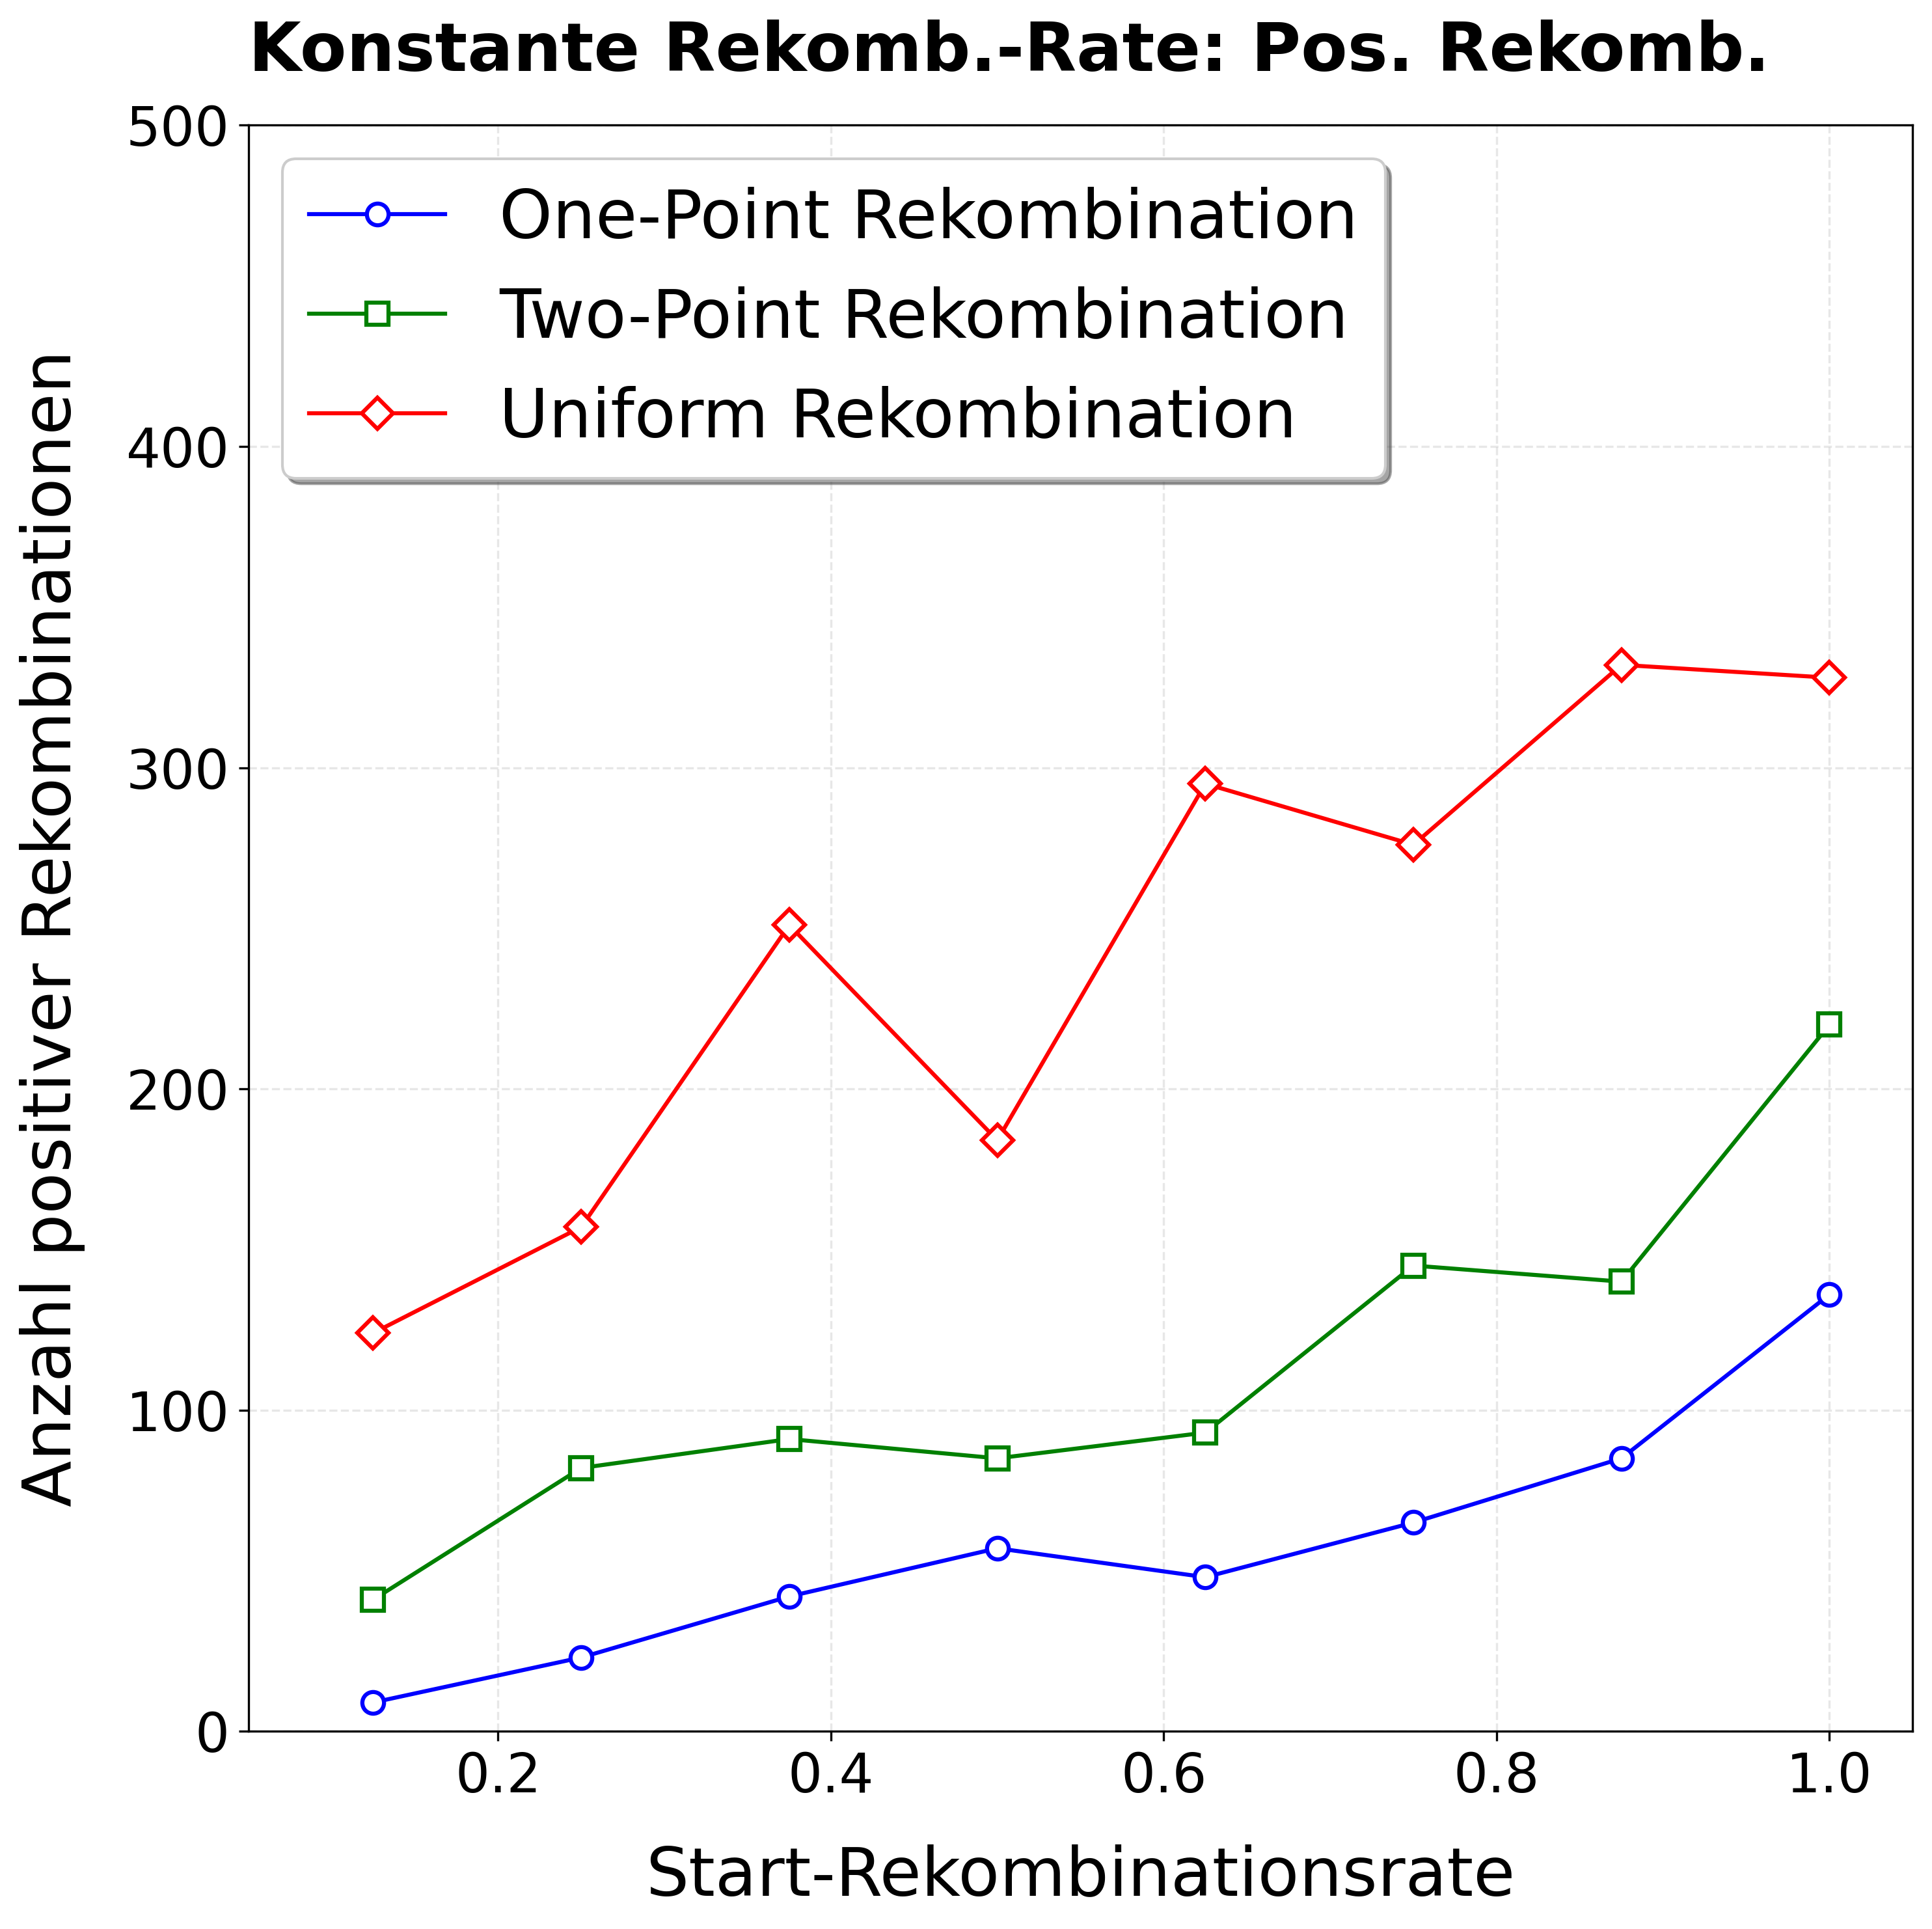
\includegraphics[width=\textwidth]{Bilder/KozaPlotPositiveRekombinationKonstant.png}
		\caption{Konstant}
		\label{fig:kozaPosRekombinationKonstant}
	\end{subfigure}%
	\hfill
	\begin{subfigure}[b]{0.32\textwidth}
		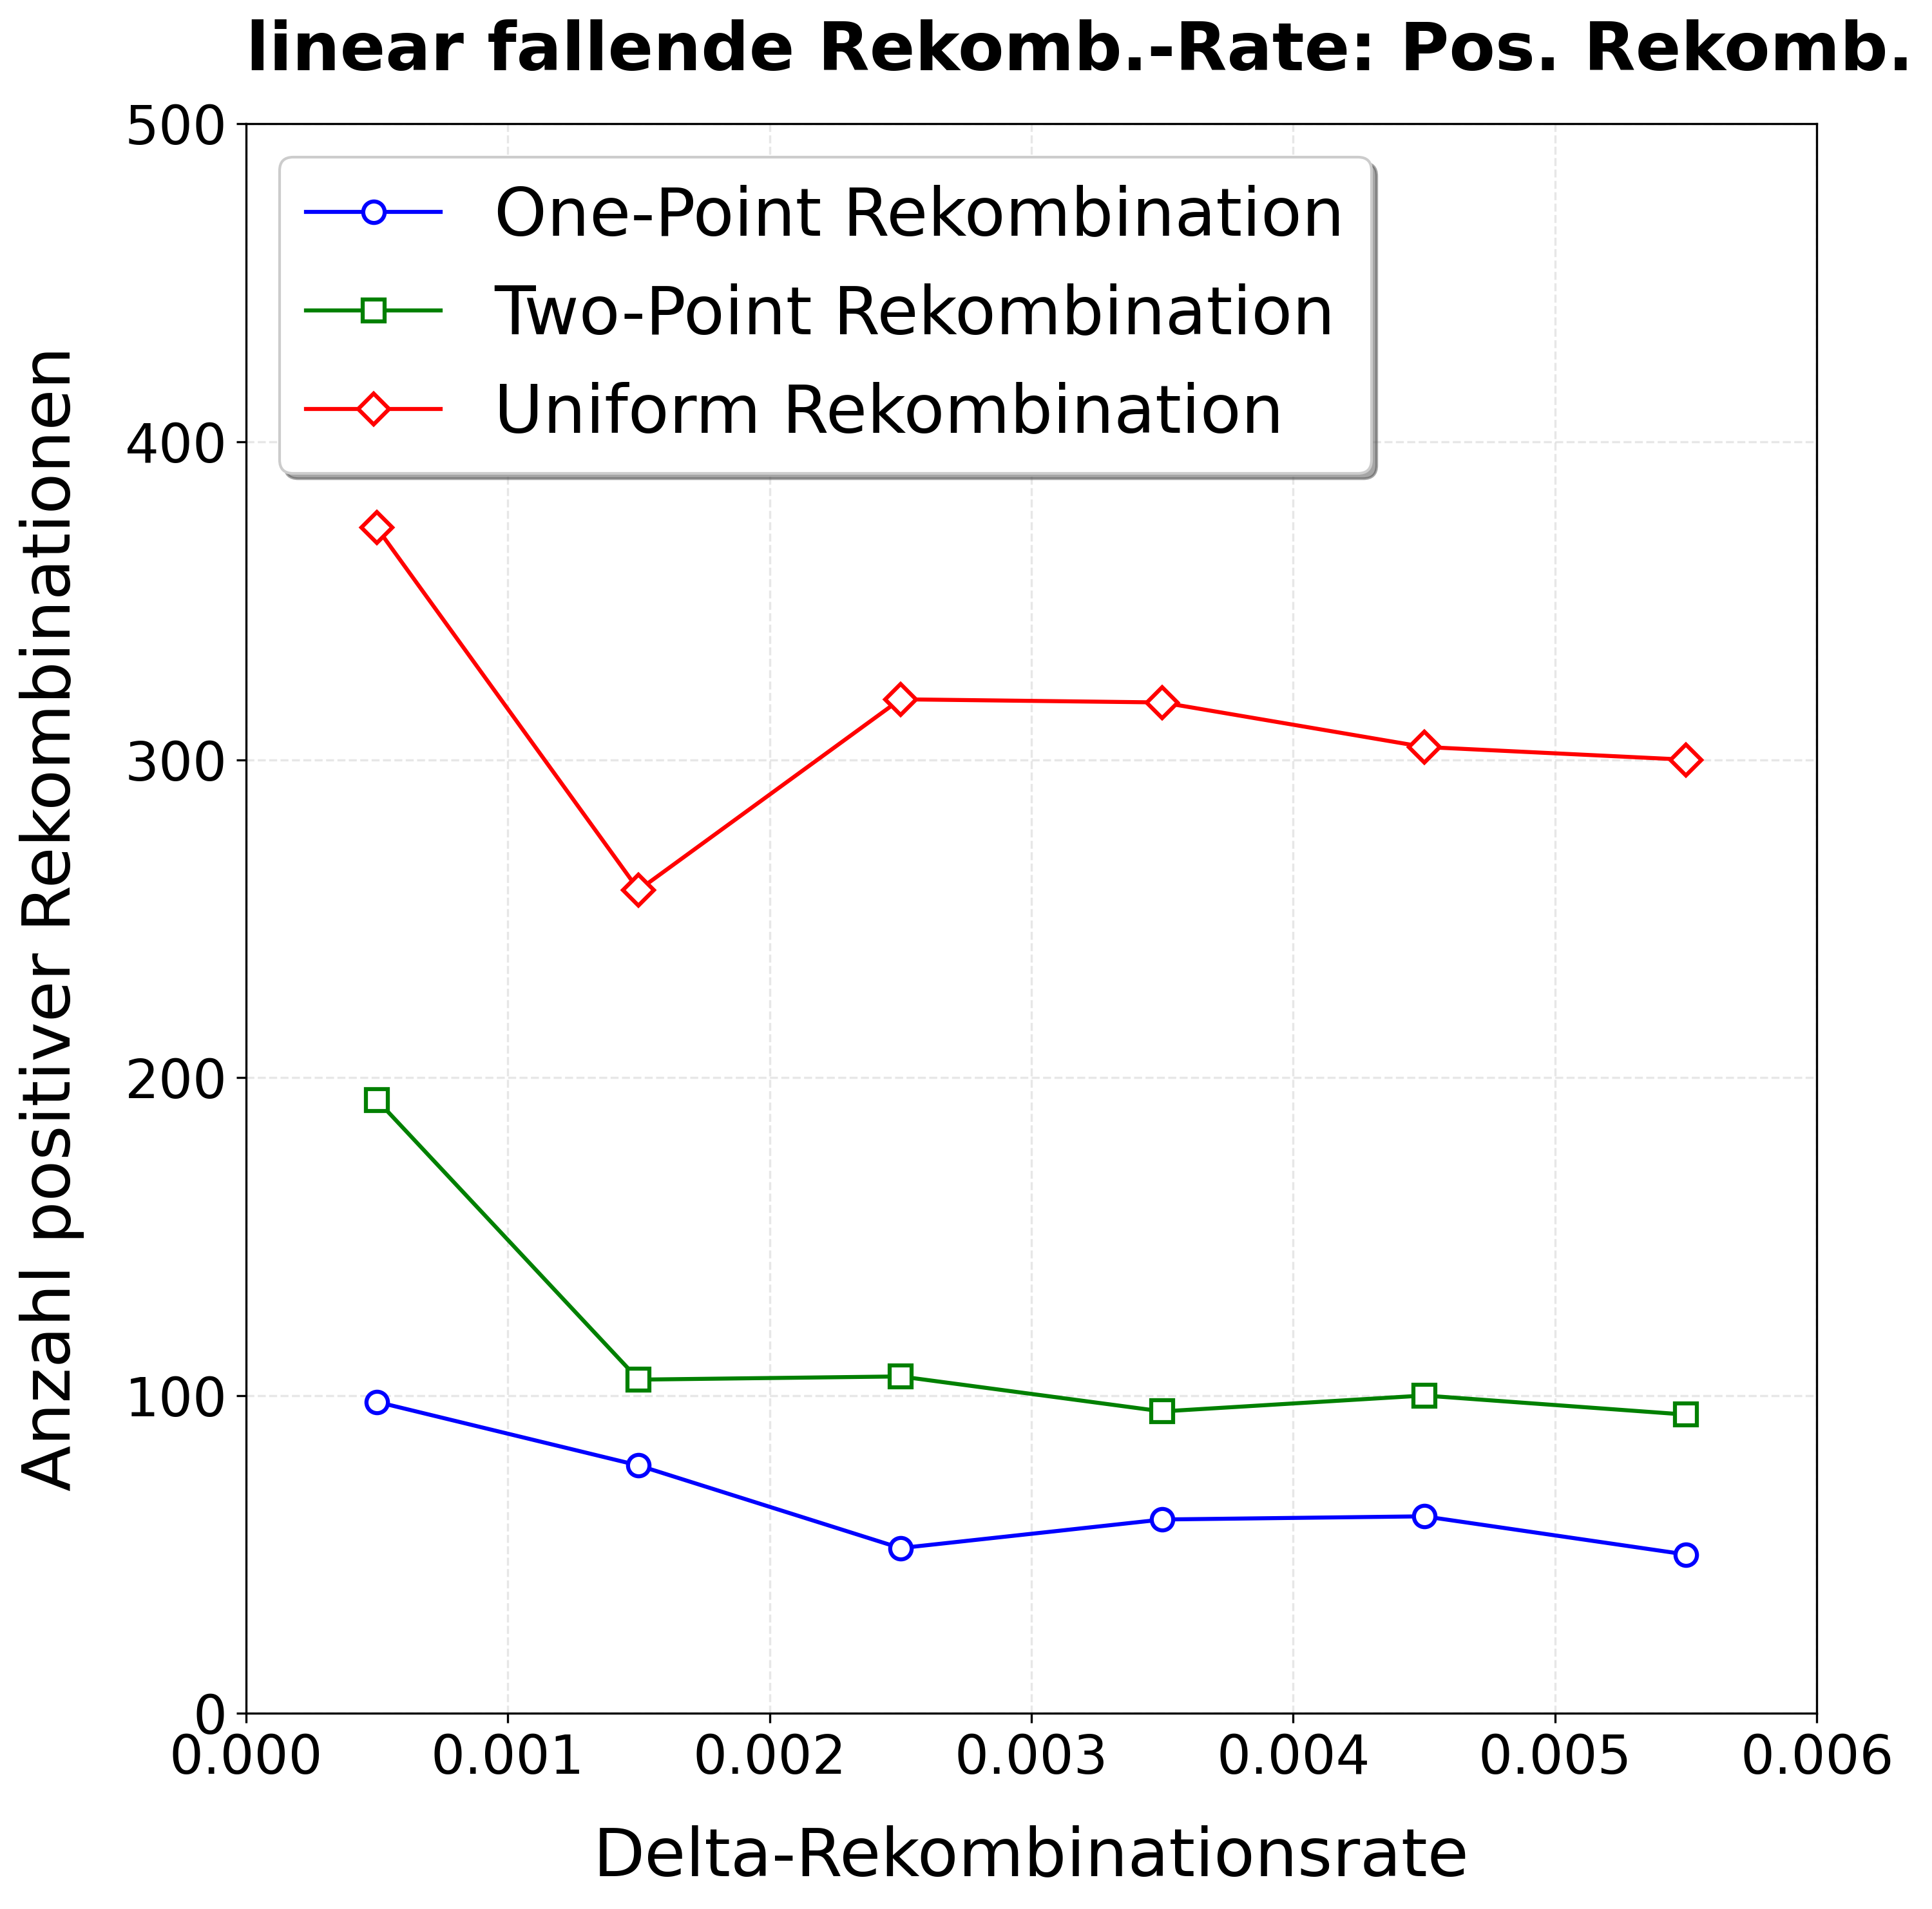
\includegraphics[width=\textwidth]{Bilder/KozaPlotPositiveRekombinationClegg.png}
		\caption{linear fallend}
		\label{fig:kozaPosRekombinationClegg}
	\end{subfigure}%
	\hfill
	\begin{subfigure}[b]{0.32\textwidth}
		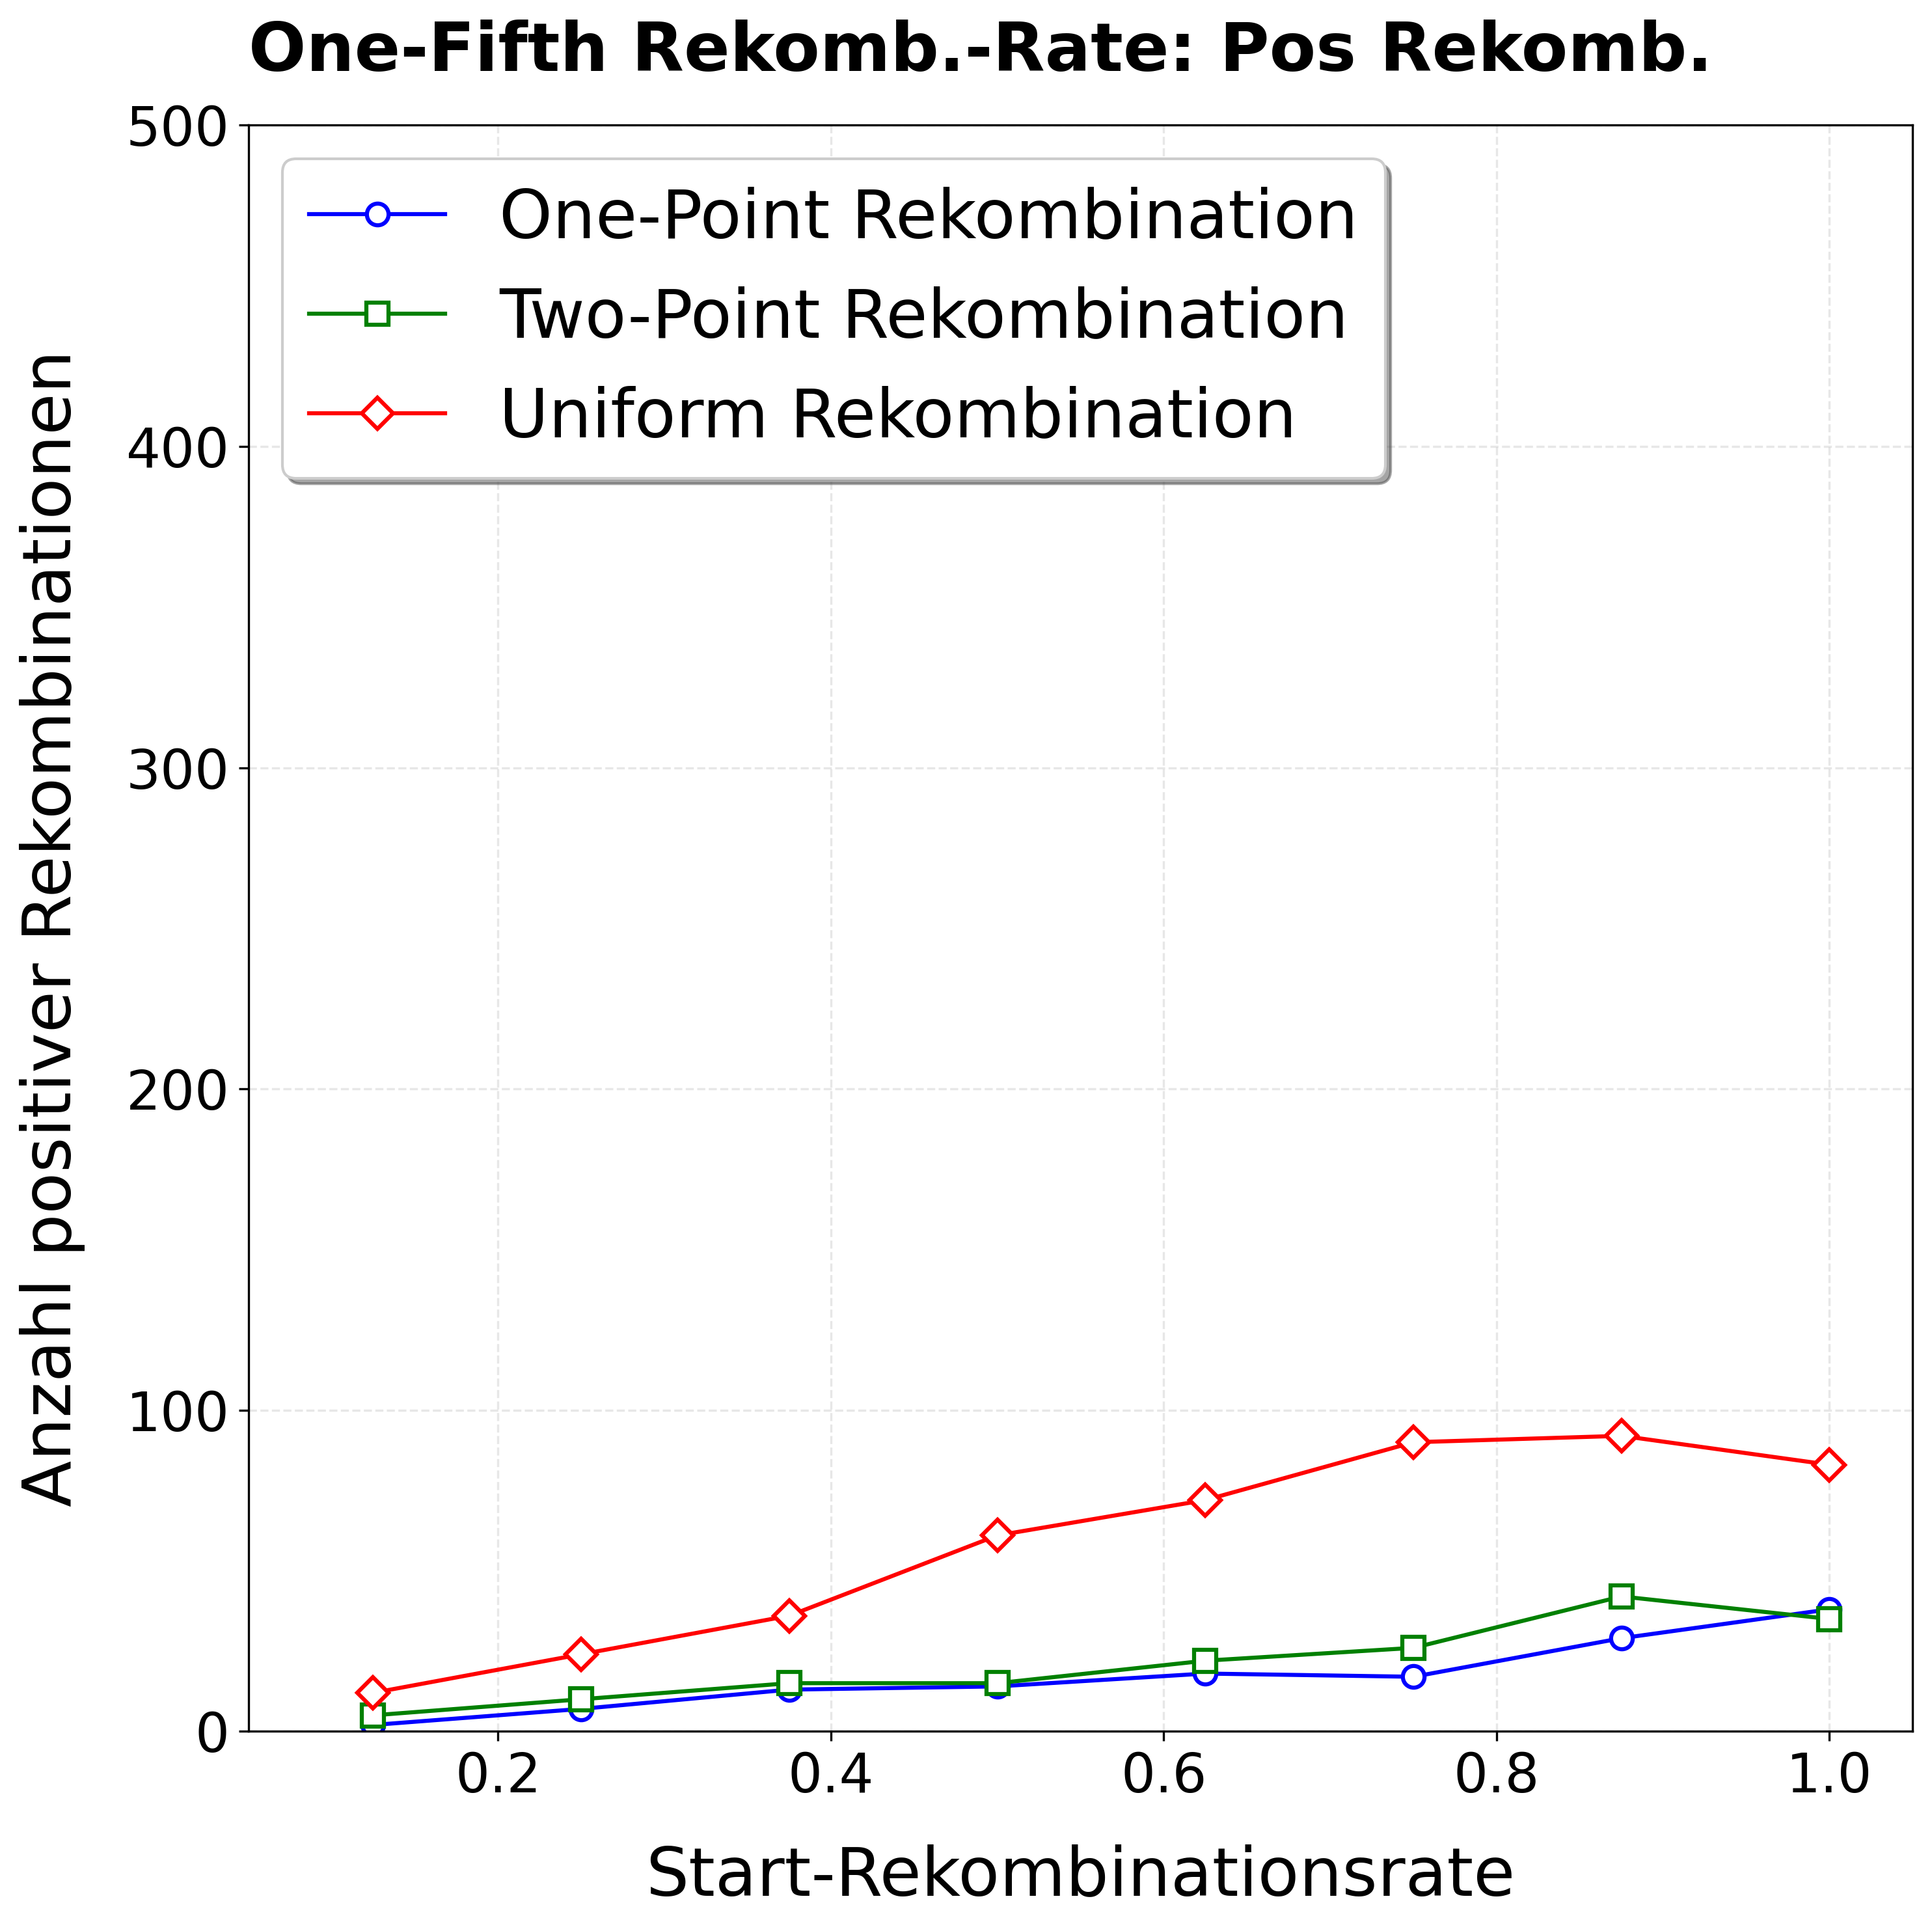
\includegraphics[width=\textwidth]{Bilder/KozaPlotPositiveRekombinationOneFifth.png}
		\caption{One-Fifth Regel}
		\label{fig:kozaPosRekombinationOneFifth}
	\end{subfigure}
	\caption{Koza: Raten-Arten und Anzahl positive Rekombinationen}
	\label{fig:kozaPosRekombination}
\end{figure}

Abbildung \ref{fig:kozaPosRekombination} beschreibt die positiven Rekombinationsraten pro CGP-Konfiguration, aufgeteilt in die verschiedenen Rekombinationsraten-Arten. 
Dabei sind die verschiedenen Rekombinationsarten mit unterschiedlichen Farben dargestellt.
Zu erkennen ist, dass die Uniform Rekombination für jede Rekombinationsraten-Art mehr positive Rekombinationen erzeugt als es die anderen Rekombinationsarten schaffen.
Die Rekombination mit der One-Fifth Regel schneidet in dieser Betrachtung schlechter ab als die konstante und linear fallende Rekombinationsrate.
Zu beachten ist, dass es sich dabei um eine quantitative Bewertung handelt.
Es wird also nicht ersichtlich wie hoch die jeweiligen Trainingserfolge der Rekombinationen ausfallen.
Es macht Sinn dies besonders für SR Benchmarks in weiteren Tests näher zu betrachten, da hier die Fitness einen kontinuierlichen Wert einnimmt und sich die Trainingserfolge stark voneinander unterscheiden können.\\
Für die konstante Rekombinationsrate und diejenige mit der One-Fifth Regel, werden mit höheren Rekombinationsraten auch höhere Chancen gegeben, dass eine Rekombination die Fitness verbessert.
Demnach macht es Sinn, dass für höhere Rekombinationsraten die Anzahl an positiven Rekombinationen steigt, wie es in den Abbildungen \ref{fig:kozaPosRekombinationKonstant} und \ref{fig:kozaPosRekombinationOneFifth} der Fall ist.
Interessant werden demnach diejenigen lokalen Maxima, die bereits entstehen, bevor jeweils die maximale Rekombinationsrate erreicht wurde.
In diesen Punkten könnte die Rekombinationsrate für diese Konfigurationen der Hyperparameter besonders gut ausfallen, da hier prozentual mehr ausgeführte Rekombinationen zu einer Verbesserung der Fitness führen.


\subsection{Rohdatenanalyse: Zusammenfassung}
\label{subsec:rohdatenZusammenfassung}

Zuerst sollen die Ergebnisse der Hyperparameteranalyse von Parity und Keijzer miteinander verglichen werden, um Zusammenhänge zu erschließen und einzelne Beobachtungen validieren zu können.
Die folgenden Abschnitte beziehen sich dabei auf die jeweiligen Spalten der Tabellen \ref{table:parityHPO} und \ref{table:keijzerHPO}.\\
\textbf{Rechenknoten:} Bei Parity kann beobachtet werden, dass die CGP-Konfiguration ohne Rekombination am wenigsten Rechenknoten aufweist. 
Außerdem kann der Trend beobachtet werden, dass komplexere Rekombinationsalgorithmen durchschnittlich weniger Rechenknoten zugeschrieben bekommen als einfachere Algorithmen.
Dabei ist die Streuung um den Mittelwert höher, umso komplexer die Rekombinationsalgorithmen sind.
Dies könnte bedeuten, dass aus einer größeren Rechenknotenanzahl eine kleinere Streuung um diese pro Rekombinationsart folgt.
Im Vergleich dazu ergeben die Ergebnisse von Keijzer ein völlig anderes Bild: gegensätzlich zu Parity hat die CGP-Konfiguration ohne Rekombination die höchste Anzahl an Rechenknoten im Vergleich zu den Mittelwerten über die unterschiedlichen Rekombinationsalgorithmen.
Den bei Parity beobachteten Trend, dass komplexere Rekombinationen eine niedrigere Anzahl an Rechenknoten erfordern könnten, kann bei Keijzer nicht bestätigt werden.
Hier wird für die Uniform-Rekombination die höchste durchschnittliche Anzahl an Rechenknoten erfordert.
Ebenso ergibt sich für Keijzer ein anderes Bild als bei Parity, wenn man die Streuung der Rechenknotenanzahl betrachtet: Die Two-Point Rekombination weist am wenigsten Rechenknoten auf, allerdings auch die geringste Streuung.
Zusammenfassend lässt sich für die Anzahl der Rechenknoten sagen, dass Parity und Keijzer vollkommen unterschiedliche Ergebnisse liefern.
Demnach können keine Aussagen getroffen werden, wie die Anzahl der Rechenknoten mit den unterschiedlichen CGP-Konfigurationen zusammenhängen.
Die Möglichkeit besteht ebenfalls, dass überhaupt kein Zusammenhang zwischen diesen beiden Komponenten besteht.
Durch weitere Tests könnte dies näher betrachtet werden.\\
\textbf{Populationsgröße:} Bei Betrachtung der Populationsgröße kann für Parity zusammengefasst werden, dass die CGP-Konfiguration ohne Rekombination die deutlich kleinste Populationsgröße benötigt hat.
Für Keijzer konnte diese Beobachtung nicht geteilt werden.
Umgekehrt konnte bei Parity nicht bestätigt werden, dass Two-Point und Uniform Rekombination mit linear fallender Rekombinationsrate ohne Offset einen geringeren $\lambda$-Wert aufweisen.
Zusammenfassend lässt sich also auch für die Populationsgröße kein Zusammenhang zu den unterschiedlichen Rekombinationsarten herstellen.\\
\textbf{Rekombinationsraten:} Bei den Ergebnissen der Hyperparameteroptimierung vom Parity-Testszenario werden von konstanten Rekombinationsalgorithmen besonders hohe und besonders niedrige Rekombinationsraten vermieden.
Für die linear fallende Rate und die Rekombinationsrate mit der One-Fifth Regel wird (nahezu) der gesamte Definitionsbereich genutzt.
Wieder im Gegensatz dazu stehen die Ergebnisse des Keijzer-Testszenarios.
Hier werden für nahezu alle CGP-Konfigurationen sehr hohe oder niedrige Werte für die Rekombinationsrate verwendet.
Somit kann durch die Ergebnisse der Hyperparameteranalyse nicht bewertet werden, welche Bereiche der Rekombinationsrate besonders effektiv sind.\\
\textbf{Offset:} Bei Parity wird der geringste Offset bei der Two-Point Rekombination und der höchste Offset bei der Uniform Rekombination verwendet.
Werden bei Keijzer die originalen Ergebnisse verwendet, bei denen ein Offset von 0 zugelassen wird, kann dieses Verhalten ebenfalls beobachtet werden.
Dies könnte bedeuten, dass die Two-Point Rekombination effizienter ist als die Uniform Rekombination, da bei ersterem weniger Rekombinationsschritte ausgesetzt werden.
Die für den Offset neu eingefügten Werte, falls ein Offset gleich 0 bestimmt wird, sind bei Parity ähnlich zum allgemeinen Mittelwert des Offsets.
Ein anderes Verhalten kann für das Keijzer-Testszenario beobachtet werden, bei dem die zweitbesten Parametersätze sehr hohe Offset-Werte verwenden.
Dies ergibt also einen extrem hohen Sprung im Offset zwischen erstbestem und zweitbestem Parametersatz.
Das ist ein Indiz dafür, dass die Güte eines CGPs nicht kausal mit der Höhe des Offsets zusammenhängt.\\
Zu beachten ist, dass die Ergebnisse der Hyperparameteranalyse mit Vorsicht zu begutachten sind.
Um die Ergebnisse und die daraus abgeleiteten Aussagen zu validieren könnte es sinnvoll sein eine umfangreichere Hyperparameteranalyse auszuführen.
Diese sollte mit Hilfe von mehr Rechenkapazität ausgeführt werden, damit mehr Hyperparameter getestet werden können.
Außerdem kann die Anzahl an ausgeführten CGP-Trainings pro Bewertungsschritt in der Hyperparameteranalyse höher gesetzt werden.
Durch diese Schritte könnten sich die Ergebnisse von Parity und Keijzer aneinander angleichen, wodurch bessere Bewertungen stattfinden könnten.
Andernfalls könnte die Aussage gestärkt werden, dass die CGP-Konfigurationen keinen Zusammenhang zur Auswahl einzelner Hyperparameter aufweisen.\\

Folgend sollen die Rohdatenanalysen der vier Testszenarien Parity, Keijzer, Encode und Koza zusammengefasst und miteinander verglichen werden.\\
Für alle Testszenarien wurde festgestellt, dass deutlich mehr Mutationen zu einer Verbesserung der Fitness geführt haben als es für Rekombinationen der Fall war.
Dies kann damit zusammenhängen, dass die Rekombinationserfolge bei allen Testszenarien in den frühen Testphasen stattgefunden haben.
Diese Beobachtung wird bei Parity und Keijzer dadurch gestützt, dass die Rekombination kein einziges mal die Fitness verbessern konnte, wenn ein Offset eingesetzt wurde.
Für die Testszenarien Keijzer und Koza wurden mehr Rekombinationserfolge aufgezeichnet als für die booleschen Probleme.
Das kann damit zusammenhängen, dass die Fitness in booleschen Problemen einen diskreten Wertebereich aufweist.
Für Tests aus der symbolischen Regression ergeben sich damit mehr Möglichkeiten die Fitness zu verbessern, indem die Verbesserungen kleinschrittiger ablaufen können.
Zu beachten ist, dass die Bewertungen in diesem Abschnitt \ref{sec:ergebnisseRohdaten} quantitativ sind und nicht qualitativ.
Dies bedeutet, dass nur betrachtet wird wie viele Rekombinationen und Mutationen die Fitness verbessert haben.
Dabei lässt sich keine Aussage darüber treffen wie groß die Rekombinations- und Mutationserfolge ausfallen.
Dies sollte in weiteren Tests näher untersucht werden, um näher beurteilen zu können wie gut die Rekombination abschneidet.\\
Im Koza-Testszenario treten vereinzelt CGP-Konfigurationen mit konstanter Rekombinationsrate auf, in denen die erfolgreichen Rekombinationen etwas später stattfinden.
Diese leicht erhöhte Iterationenzahl hat allerdings keinen Zusammenhang zu der Anzahl an Iterationen bis zur Konvergenz.
Demnach ist es unwahrscheinlich, dass die Rekombinationserfolge nur später auftreten, weil das Training an sich länger lief.
Ein Zusammenhang zwischen den späteren Rekombinationserfolgen und der konstanten Rekombinationsrate kann nicht vollends bestätigt werden und kann in weiteren Tests näher untersucht werden.
Falls dieser oder ein ähnlicher Zusammenhang festgestellt werden kann, könnte die Rekombination gezielter verwendet werden.
So könnte beispielsweise die linear fallende Rekombinationsrate verwendet werden, die ähnliche Anzahlen einer positiven Rekombination aufweisen, allerdings frühere Rekombinationserfolge bietet.
So könnte die Rekombination früher ausgesetzt werden, ohne Erfolge der Rekombination einzubüßen.
Allerdings wird beim Encode-Testszenario so ein Fall mit späteren Rekombinationserfolgen nicht auf.
Dies kann aber daran liegen, dass im Encode-Testszenario insgesamt weniger Rekombinationserfolge vermerkt wurden als beim Koza-Testfall.
Es ist also empfohlen dieses Verhalten bei weiteren Testfällen mit SR zu prüfen.\\
Ein weiterer Punkt, der für alle Testszenarien beobachtet wurde ist, dass es Iterationen gibt, in denen die verbesserte Fitness durch die Mutation verloren gegangen ist.
Dies kann auftreten, da die Auswahl der Elitisten erst nach der Rekombination ausgeführt wird und somit im Normalfall keine Evaluation nach der Rekombination und vor der Mutation stattfindet.
Dieser Missstand könnte dadurch gelöst werden, indem die Fitness bereits nach der Rekombination evaluiert wird und hier bereits Elitisten zwischengespeichert werden.
Anschließend könnten die Elitisten nach der Mutation mit ersteren verglichen werden, um so die besten Elitisten zu wählen.\\
Des weiteren fällt auf, dass die CGP-Konfigurationen mit Rekombination nur gelegentlich eine schnellere Konvergenz erzielen, obwohl neben der Mutation auch die Rekombination die Fitness verbessert.
In den Testfällen Encode und Koza konnte außerdem festgestellt werden, dass die Spalten, die die Rekombination beschreiben keine zusammenhängenden Muster zu den Ergebnis-Spalten aufweisen.
In den Hyperparameteranalysen von Parity und Keijzer werden außerdem jeweils 7 aus 9 CGP-Konfigurationen mit einem Offset versehen und so der gesamte Rekombinationserfolg übergangen.
Für den Keijzer-Testfall konnte auch beobachtet werden, dass diejenigen CGP-Konfigurationen mit Offset weniger Iterationen bei konvergierenden Durchgängen brauchten als die jeweiligen gleichen CGP-Konfigurationen ohne Offset.
Dies könnte ein Indiz dafür sein, dass nicht nur die Mutation die Rekombination negativ beeinflusst, sondern auch andersherum die Rekombinationen den Erfolg der Mutationen verringert.
Eine Lösungsmöglichkeit wäre womöglich eine Spaltung von Rekombination und Mutation.
Dabei würden die beiden genetischen Operatoren nicht nacheinander ablaufen, sondern gleichzeitig.
Dafür könnte die Population gespalten werden und ein Teil des Nachwuchs durch Rekombination und der andere Teil durch Mutation erzeugt werden.
So würden gleichzeitig die großen Veränderungen der Chromosome eingebracht werden, die die Rekombination erzeugt, aber auch die kleineren Anpassungen, die aus der Mutation herrühren.
So könnte der Lösungsraum gleichzeitig groß- und kleinschrittig abgesucht werden.\\
Als letzte wichtige Erkenntnis aus diesem Abschnitt kann zusammengefasst werden, dass die Uniform Rekombination deutlich mehr positive Rekombinationen hervorgebracht hat als die anderen Rekombinationsarten.
Während die konstante und linear fallende Rekombination ähnlich viele Rekombinationserfolge erzielt haben, hat die Rekombination mit One-Fifth Regel in deutlich weniger Iterationen die Fitness verbessert.
Demnach hat die Uniform Rekombination mit konstanter oder linear fallender Rekombinationsrate das größte Potential die Rekombination an sich effizienter zu gestalten.
Interessant ist die Beobachtung, dass nicht nur höhere Rekombinationsraten zu mehr positiven Rekombinationen geführt haben, obwohl eine höhere Rekombinationsrate die Wahrscheinlichkeit für eine effiziente Rekombination steigert.
Im Keijzer-Testszenario konnte die konstante Rekombinationsrate von 0,8 mehr positiver Rekombinationen erzielen als die linear fallende Rekombinationsrate, die mit 0,9 initialisiert wird.
Auch bei den Testfällen Encode und Koza konnten in den Plots zu positiven Rekombinationen über Rekombinationsraten lokale Maxima gefunden werden.
Bei diesen wurden Hochpunkte für positive Rekombinationen gefunden, die bei relativ geringen Rekombinationsraten entstanden sind.
Diese Rekombinationsraten könnten weiter in anderen Testszenarien untersucht werden, um Muster zu erkennen und gegebenenfalls eine ideale Rekombinationsrate zu finden oder mehr Verständnis aufzubauen.\\
Die Ergebnisse in diesem Abschnitt zeigen, dass im Gebrauch der Rekombinationsalgorithmen mehr Potential steckt als mit dem CGP-Aufbau Abbildung \ref{fig:aufbauCGP} genutzt wird.
Der in diesem Abschnitt erläuterte Ausblick kann verwendet werden, um weitere Erkenntnisse zu sammeln und die Rekombination im allgemeinen weiter zu fördern.
Trotzdem, dass das Potential nicht voll genutzt wird, konnten die bisherigen Ergebnisse Grund zu der Vermutung geben, dass bereits mit diesem Stand die Effizienz eines CGPs gesteigert werden kann, wenn die Rekombination richtig gewählt und parametriert wird.
Diese Ergebnisse wurden für Encode und Koza auch erzielt, obwohl nur die Hyperparameter der CGP-Konfigurationen ohne Rekombination optimiert wurden.
Die folgenden Abschnitte \ref{sec:ergebnisseBayes} und \ref{sec:ergebnissePlots} werten den Ist-Stand der Standard-Rekombination in CGPs weiter aus.


\section{Ergebnisse Bayes'sche Analyse}
\label{sec:ergebnisseBayes}

In diesem Abschnitt werden die Ergebnisse der bayes'schen Analyse aufgezeigt und bewertet.
Dafür werden die Tabellen aus dem Anhang \ref{sec:appendixTabellenBayes} verwendet.
Aus den Ergebnissen der Rohdatenanalyse von Encode (Abschnitt \ref{subsec:rohdatenEncode}) und Koza (Abschnitt \ref{subsec:rohdatenKoza}) geht hervor, dass für Encode die Fitness bei der 10000. Iteration bewertet wird und für Koza die Anzahl der Iterationen bis zur Konvergenz.
Für die restlichen Testszenarien Parity und Keijzer wird ebenfalls die Anzahl der Iterationen bis zur Konvergenz analysiert.
Ziel der bayes'schen Analyse ist es herauszufinden, ob Rekombination die Effizienz von CGPs verbessern.
Aus Abschnitt \ref{subsec:rohdatenZusammenfassung} geht hervor, dass Rekombination ein vermutlich größeres Potential besitzt als mit Standard-Vorgehensweisen genutzt wird.
Die bayes'sche Analyse wird verwendet, um die Effizienz der Standard-Vorgehensweisen mit und ohne Rekombination abzugleichen.\\
Folgend werden die Spalten der Tabellen näher erläutert:\\
\textbf{CGP-Konfiguration:} Es handelt sich um die jeweils für das Training verwendete CGP-Konfiguration.
Für Parity und Keijzer sind das die durch die Hyperparameteranalyse optimierten CGP-Konfigurationen mit und ohne Offset.
Bei Encode und Koza wird der Offset wie in den Abschnitten \ref{subsec:rohdatenEncode} und \ref{subsec:rohdatenKoza} beschrieben kein Offset betrachtet.
Dafür werden jeweils verschiedene Belegungen der Rekombinationsraten analysiert.\\
\textbf{HPDI (Iter. / Fitn.):} Diese Spalte gibt den HPDI von 95\% an.
\glqq Iter.\grqq\space und \glqq Fitn.\grqq\space gibt dabei an, ob dabei die Fitness oder die Anzahl der Iterationen bewertet werden.
Die HPDI-Berechnung kann ebenfalls mit zensierten Werten umgehen.
Dies wird für die Analyse der Iterationen bis zur Konvergenz relevant.
Dabei wird dem Modell mitgegeben wie viele CGP-Modelle nicht konvergiert sind und bei welcher Iteration ungefähr alle Durchläufe das Stopp-Kriterium erfüllen.
Diese Bewertung enthält demnach Schätzwerte und sind mit Vorsicht zu bewerten.
Die Schätzwerte bewerten wie hoch die Fitness zur Abbruchiteration ist und lassen diese Information in die Schätzung einfließen.
Da für alle bewerteten CGP-Konfigurationen das gleiche Verfahren angewendet wurde, sollten die Ergebnisse allerdings miteinander vergleichbar sein können.\\
\textbf{MW:} Diese Spalte gibt den Mittelwert der gefitteten Wahrscheinlichkeitsverteilung an.\\
\textbf{PL-Platz:} Dabei handelt es sich um die Platzierung der CGP-Konfigurationen mit Hilfe des Plackett-Luce-Modells.
Die Platzierung gibt eine Wahrscheinlichkeit an, dass die jeweilige CGP-Konfiguration die besten Ergebnisse liefert.
Demnach werden Werte von 0 bis 1 vergeben, die zusammen 100\% ergeben.
Das Plackett-Luce-Modell kann mit einer Zensur der Daten nicht umgehen.
Deswegen wurden dem Modell die jeweils vorliegenden Ergebnissen zur Abbruchiteration mitgegeben.


\subsection{Bayes'sche Analyse: Parity}
\label{subsec:bayesParity}

Dieser Abschnitt bezieht sich auf die Tabelle \ref{table:parityBayesian} und bewertet lediglich die Ergebnisse der bayes'schen Analyse von Parity.
Jegliche Aussagen können noch nicht auf die Allgemeinheit geschlossen werden und werden in Abschnitt \ref{subsec:bayesZusammenfassung} näher bewertet.\\
Werden die MW der verschiedenen CGP-Modelle betrachtet, wird deutlich, dass nur 2 der 18 CGP-Konfigurationen mit Rekombination schlechter abschneiden als diejenige ohne Rekombination.
Das ist ein Zeichen dafür, dass Rekombination durchaus die Effizienz von CGP steigern kann, wenn die Rekombination sinnvoll konfiguriert wird.\\
Die jeweils drei niedrigsten MW und drei höchsten PL-Plätze sind in der Tabelle \ref{table:parityBayesian} grün markiert, während die drei höchsten MW und drei niedrigsten PL-Plätze rot sind.
Zu sehen ist, dass die MW und PL-Plätze nicht genau die gleichen CGP-Konfigurationen als gleich gut oder schlecht bewerten.
Dies kann daher rühren, dass in die Berechnung der MW die Schätzwerte einfließen, wann ein CGP-Modell konvergiert.
Für die Berechnung der PL-Plätze ist das nicht der Fall.
Die MW geben also mehr Eindrücke daraus wie nah die CGP-Modelle an der Konvergenz sind, wenn sie das Stopp-Kriterium noch nicht erfüllt haben.
Allerdings handelt es sich dabei wie bereits erwähnt um einen Schätzwert, der durchaus mit Vorsicht betrachtet werden muss.
Die Tabelle zeigt aber, dass die Trends ob eine CGP-Konfiguration gute oder schlechte Ergebnisse hervorbringt durch MW und PL-Plätze gleich bewertet werden.
Bei den Unterschieden handelt es sich nur um einzelne Platzierungen der CGP-Konfigurationen.
Durch die gemeinsame Betrachtung von MW und PL-Plätze kann demnach ein gutes Bild davon gegeben werden wie effizient einzelne CGP-Modelle trainieren.
Werden die besten und schlechtesten MW und PL-Plätze in der Tabelle betrachtet, wird deutlich, dass die CGP-Konfigurationen mit der One-Point Rekombination deutlich bessere Ergebnisse liefert als die anderen Rekombinationsarten.
Da aus Abschnitt \ref{subsec:rohdatenParity} bekannt ist, dass für die One-Point Rekombination deutlich weniger Rekombinationserfolge auftreten als bei den anderen Rekombinationsarten, kann davon ausgegangen werden, dass bei bei diesen CGP-Konfigurationen die Rekombination weniger Einfluss auf den Erfolg des Trainings hat.
Vergleicht man die schlechtesten Verfahren nach MW und PL-Plätzen mit Rekombination ohne Offset aus Tabelle \ref{table:parityBayesian} mit der Tabelle \ref{table:parityRohdaten} kann beobachtet werden, dass der Anteil der negativen Mutationen pro positive Rekombinationen relativ hoch ist.
Das kann dafür sprechen, dass Rekombination mit dem Standard-CGP-Verfahren mit weniger einflussreicher Rekombination besser funktioniert, da Rekombination und Mutation nicht ausreichend aneinander abgestimmt sind und damit einflussreichere Rekombination (mit mehr möglichen positiven Rekombinationsschritten) weniger gute Ergebnisse liefern.
Wenn dieser Ansatz der Realität entspricht, könnte demnach durch eine Anpassung des CGP-Verfahrens Rekombination sinnvoller eingesetzt werden, sodass einflussreichere Rekombinationsarten wie die Uniform Rekombination einen größeren Mehrwert generieren.\\
Des weiteren werden die Ergebnisse jeweils bezüglich MW und PL-Plätzen von Verfahren mit Offset mit den Ergebnissen der jeweils gleichen CGP-Konfigurationen ohne Offset verglichen.
Dabei weisen jeweils sechs aus neun CGP-Konfigurationen ohne Offset bessere Ergebnisse auf als diejenigen mit Offset.
Dies spricht dafür, dass ein Rekombinationsoffset der Effizient eines CGP-Modells schadet.
Ein Grund dafür könnte sein, dass damit die positiven Einflüsse der Rekombination gestrichen werden, während die nachteiligen Effekte des Zusammenspiels von Rekombination und Mutation weiterhin bestehen bleiben.\\
Analysiert werden nun die HPDI-Werte aus Tabelle \ref{table:parityBayesian}.
Dabei werden die HPDI-Werte mit dem kleinsten Umfang grün markiert und die mit dem größten rot.
Diese werden verwendet, um die Ergebnisse stichprobenartig zu bewerten.
Es fällt auf, dass auch was den HPDI-Umfang betrifft, die One-Point Rekombination die besten drei Werte beinhaltet.
Wenn aus allen HPDI-Werten die unteren Grenzen betrachtet und verglichen werden, kann außerdem beobachtet werden, dass die drei kleinsten unteren Grenzen Teil der grün markierten HPDIs sind.
Umgekehrt lässt sich beobachten, dass besonders große untere Grenzen zu großen Umfängen der HPDI führen.
Bei den drei größten unteren Grenzen ist dies in einem Fall keine rot markierte HPDI, allerdings handelt es sich dabei um einen ähnlich großen HPDI-Umfang, wodurch ein Trend erkennbar wird.
Dieses Verhalten weist darauf hin, dass frühe Konvergenz der frühesten erfolgreichen Trainings ein Anzeichen dafür ist, dass die meisten CGP-Modelle relativ früh konvergieren.
Zu beachten ist, dass es sich hierbei nicht um Ausreißer handeln darf, da diese in der 95\%-igen HPDI nicht erfasst werden.
Wenn diese Beobachtung zutrifft, heißt das, dass frühe Trainingserfolge besonders wichtig sind, wenn man eine verlässliche CGP-Konfiguration generieren möchte, deren Modelle in einer relativ kleinen Iterationsspanne konvergieren sollen.
Da Rekombination laut Abschnitt \ref{subsec:rohdatenZusammenfassung} in früheren Iterationen ein besonders hohes Potential aufweist, ist es demnach sinnvoll die Rekombination und deren Einsatz effizienter zu gestalten.

\subsection{Bayes'sche Analyse: Keijzer}
\label{subsec:bayesKeijzer}

Dieser Abschnitt beurteilt die bayes'sche Analyse des Keijzer-Testszenarios und bezieht sich dabei auf die Tabelle \ref{table:keijzerBayesian}.
Im ersten Schritt wird der MW aller CGP-Konfigurationen bewertet.
Bei sechs aus 18 Verfahren mit Rekombination sind die MW kleiner als die der CGP-Konfiguration ohne Rekombination.
Bei Betrachtung der Mittelwerte der Spalte MW über die verschiedenen Rekombinationsarten hinweg ergeben sich folgende Werte: One-Point Rekombination braucht durchschnittlich ca. 8200 Iterationen, Two-Point ca. 8670 und Uniform ungefähr 8650.
Damit liegen alle Mittelwerte unterhalb von ca. 9552 Iterationen, die das CGP-Modell ohne Rekombination benötigt.
Das heißt, dass es sich beim Standard-CGP-Vorgehen im Durchschnitt lohnt Rekombination anzuwenden.\\
Die jeweils drei besten MW und PL-Plätze sind in der Tabelle grün markiert, während die schlechtesten rot sind.
Zu beobachten ist, dass sich die jeweils besten und schlechtesten Werte der beiden Spalten nicht immer entsprechen.
Dies ist der Fall, da bei den PL-Plätzen keine Schätzung darüber abgegeben wird, wann nicht-konvergente CGP-Modelle das Stopp-Kriterium erfüllen. 
Hier wird nur die maximale Iterationsgrenze (6500 Iterationen) angegeben, falls ein CGP-Modell nicht fertig trainiert wurde.
Demnach fängt die Spalte MW besser ein wie hoch die Fitness bei Abbruch des CGP-Trainings war.
Allerdings gibt es bei der Schätzung der Iterationen eine gewisse Unsicherheit darüber, wie sich die Ergebnisse der CGP-Modelle entwickeln.
Deswegen werden beide Spalten in die Bewertung einbezogen.
Zu sehen ist, dass die schlechtesten Ergebnisse von MW und PL-PLatz in den Rekombinationsraten Two-Point und Uniform auftreten.
Die besten Ergebnisse treten allerdings auch vor allem in diesem Rekombinationsarten auf, was aufzeigt wie wichtig es ist nicht nur die Rekombinationsart richtig zu wählen, sondern auch die Rekombinationsraten-Arten und deren Parametrierungen abzuwägen.\\
Wird ein näherer Blick auf diejenigen CGP-Konfigurationen aus Tabelle \ref{table:keijzerRohdaten} mit Rekombination und ohne Offset geworden, bei denen die Spalten MW und PL-Platz aus Tabelle \ref{table:keijzerBayesian} besonders gut oder besonders schlecht ausfallen, fällt auf, dass die schlechten Ergebnisse vor allem bei denjenigen CGP-Konfigurationen auftreten, in denen an sich viele negative Mutationen auftreten (Two-Point Clegg und Uniform Konstant).
Dies kann bedeuten, dass in diesen CGP-Modellen die Rekombination und Mutation häufiger gegeneinander gearbeitet haben als gemeinsam bessere Ergebnisse zu liefern.
Die besseren Ergebnisse nach MW und PL-Plätzen treten in denjenigen Konfigurationen auf, in denen die positiven Rekombinationserfolge entweder relativ selten auftreten oder in denen die negativen Mutationen anteilig weniger auftreten (One-Point Konstant und Uniform One-Fifth).
Das könnten diejenigen CGP-Konfigurationen sein, in denen die Rekombination weniger einflussreich ist oder sich die Rekombination und Mutation weniger negativ beeinflussen.
Da bei der CGP-Konfiguration \glqq Uniform One-Fifth ohne Offset\grqq\space in Tabelle \ref{table:keijzerRohdaten} eine sehr frühe Iterationenzahl für positive Rekombination erfasst werden kann, kann es sein, dass die Rekombination anschließend mit Hilfe der One-Fifth Regel so reduziert werden konnte, dass die Mutation anschließend nicht mehr negativ beeinflusst werden konnte.
Dieses Szenario ist kann allerdings mit den vorliegenden Daten untersucht demnach nicht evaluiert werden.\\
Des weiteren werden alle Ergebnisse aus MW und PL-Plätzen derjenigen CGP-Kon\-fi\-gu\-ra\-tionen mit Offset mit den Ergebnissen der gleichen Konfigurationen ohne Offset verglichen.
Für den MW sind die Ergebnisse von sechs aus neun Konfigurationen ohne Offset besser.
Werden die PL-Plätze bewertet sind es nur 5 aus 9.
Die Ergebnisse zeigen, dass es im Durchschnitt besser ist die Rekombination nicht auszusetzen.
Trotzdem zeigen diese Ergebnisse auch, dass das Potential von Rekombination noch weiter ausgebaut werden muss, um eine verlässliche Lösung anzubieten, bei der kein Offset mehr benötigt wird.\\
Für die nähere Betrachtung der HPDI-Werte aus Tabelle \ref{table:keijzerBayesian} werden die drei HPDI-Ranges mit dem geringsten Umfang grün markiert, während diejenigen mit dem größten Umfang rot markiert werden.
Es fällt auf, dass die Uniform Rekombination relativ kleine HPDI-Ranges aufweist, bis auf die zwei sehr großen Umfänge.
Die One-Point Rekombination weist zwei sehr geringe HPDI-Umfänge auf, während die restlichen relativ hoch ausfallen.
In der näheren Analyse wurde kein Grund gefunden, wieso gerade diese CGP-Konfigurationen so niedrige oder hohe HPDI-Ranges aufweisen. 
Werden die drei höchsten unteren Grenzen der HPDI-Werte gesammelt, fällt auf, dass diese zu den HPDI-Werten mit den größten Umfängen gehören.
Wenn umgekehrt die niedrigsten unteren Grenzen gesammelt werden, passen zwei von drei zu den HPDI-Werten mit den geringsten Umfängen, während der dritte einen ähnlich kleinen HPDI-Umfang aufzeigt.
Dies zeigt, dass wie bereits in \ref{subsec:bayesParity} erläutert, frühe Konvergenzen zu einem kleineren HPDI-Umfang führen.
So ist es zum Beispiel unwahrscheinlich, dass ein CGP bei mehreren Durchläufen relativ lange bis zur Konvergenz braucht aber dafür alle Durchläufe ähnlich lange benötigen.
Demnach ist es wichtig frühe Iterationen sinnvoll für das Training zu nutzen, um eine verlässliche Konvergenzrate zu erzielen.
Da Abschnitt \ref{subsec:rohdatenZusammenfassung} zufolge die Rekombination besonders in frühen Iterationen Potential aufzeigt, ist es umso wichtiger die Rekombination effizienter zu gestalten.


\subsection{Bayes'sche Analyse: Encode}
\label{subsec:bayesEncode}

Dieser Abschnitt befasst sich mit der Evaluierung der bayes'schen Analyse von Encode und bezieht sich auf die Tabellen \ref{table:encodeOnePointBayesian}, \ref{table:encodeTwoPointBayesian} und \ref{table:encodeUniformBayesian}.
In der bayes'schen Analyse von Encode wird bewertet wie hoch die Fitness-Werte der CGP-Modelle bei der 10000. Iteration sind.
Zu beachten ist, dass sich die Aussagen innerhalb dieses Abschnittes nur auf den Encode-Testfall beziehen und vorerst keine allgemeinen Schlussfolgerungen zulassen.
In Abschnitt \ref{subsec:bayesZusammenfassung} werden alle Ergebnisse der bayes'schen Analysen zusammengetragen und miteinander abgeglichen.\\
Innerhalb der Tabellen \ref{table:encodeOnePointBayesian}, \ref{table:encodeTwoPointBayesian} und \ref{table:encodeUniformBayesian} wurden die besten drei Ergebnisse pro Spalte grün markiert und die schlechtesten rot.
Zu beachten ist, dass die CGP-Konfiguration ohne Rekombination durch eine Hyperparameteranalyse optimiert wurde.
Die restlichen CGP-Konfigurationen haben die Hyperparameter übernommen und die Rekombinationsrate belegt.\\
Werden die MW der CGP-Konfigurationen verglichen, kann beobachtet werden, dass für die One-Point und Uniform Rekombination jeweils 20 der 22 Verfahren mit Rekombination eine bessere Fitness aufweisen als die CGP-Konfiguration ohne Rekombination.
Für die Two-Point Rekombination sind alle Verfahren schlechter, wenn Rekombination ausgeführt wird.
Werden die Mittelwerte der Spalte MW über jede Rekombinationsraten-Art gebildet, folgt folgende Tabelle \ref{table:encodeMW}:

\begin{table}[H]
	\centering
	\begin{tabular} {c | c | c | c}
		& \textbf{Konstant} & \textbf{Clegg} & \textbf{One-Fifth} \\
		\hline
		\textbf{One-Point Rekombination} & 0,03967 & 0,04082 & 0,03803\\
		\hline
		\textbf{Two-Point Rekombination} & 0,05690 & 0,05618 & 0,05387\\
		\hline
		\textbf{Uniform Rekombination} & 0,03858 & 0,03582 & 0,03748\\
	\end{tabular}
	\caption{Encode: Durchschnittliche Fitness nach 10000. Iteration}
	\label{table:encodeMW}
\end{table}

Aus den durchschnittlichen Fitness-Werten nach der 10000. Iteration folgt, dass für den Encode-Testfall die Two-Point Rekombination deutlich schlechtere Ergebnisse liefert als die anderen Rekombinationsarten.
Für jede Rekombinationsraten-Art bietet die Uniform Rekombination die besten Ergebnisse.
Werden die Rekombinationsraten-Arten für bewertet, ist für die One-Point Rekombination ist die One-Fifth Rekombinationsrate die beste, anschließend die konstante Rekombinationsrate und zuletzt die linear fallende.
Die Two-Point Rekombination weißt sehr ähnliche Werte für alle Rekombinationsraten auf.
Will man diese trotzdem in eine Reihenfolge bringen, ergibt sich die folgende: One-Fifth, linear fallend, konstant.
Bei der Uniform Rekombination ist die linear fallende Rekombinationsrate die beste, es folgt die One-Fifth Rekombinationsrate und anschließend die konstante Rekombinationsrate.
Es lässt sich also keine einheitliche Reihenfolge bilden, die die Effizienz der Rekombinationsraten-Arten abbildet.
Ebenfalls lassen sich durch die Auswertung der gesamten Tabellen keine Muster finden wie die verschiedenen Rekombinationsraten-Arten am besten zu parametrieren sind.
Dementsprechend wäre es für das Standard-CGP-Verfahren empfehlenswert verschiedene Rekombinationsraten-Arten innerhalb der Hyperparameteranalyse zu testen.\\
Für die Testszenarien Parity und Keijzer wurde in den Evaluationen der bayes'schen Analyse in den Abschnitten \ref{subsec:bayesParity} und \ref{subsec:bayesKeijzer} herausgefunden, dass kleine untere Grenzen in den HPDI-Werten sehr wahrscheinlich eine kleine Intervallgröße hervorbringen.
Bei diesen bayes'schen Analysen wurde allerdings die Anzahl der Iteration bis zur Konvergenz betrachtet, nicht so wie bei Encode, bei dem die Fitness zu einer bestimmten Iteration betrachtet wird.
Demnach soll diese Beobachtung für den Fall der Fitness-Bewertung auch betrachtet werden.
Allerdings fällt bei der Betrachtung der Tabelle \ref{table:encodeTwoPointBayesian} auf, dass diese Beobachtung für die Fitness-Bewertung nicht zutrifft:
Ein Gegenbeispiel ergeben die drei fett gedruckten HPDI-Werte dieser Tabelle, die alle drei die kleinsten untersten Grenzen abbilden.
Diese kleinen unteren Grenzen führen allerdings zu relativ großen HPDI-Ranges.
Dementsprechend kann keine Aussage darüber gemacht werden die gut die Fitnesswerte der anderen Durchläufe zu einer bestimmten Iteration sind, wenn bereits bekannt ist, dass einige Fitness-Werte sehr klein sind.


\subsection{Bayes'sche Analyse: Koza}
\label{subsec:bayesKoza}

Dieser Abschnitt evaluiert die Ergebnisse der bayes'schen Analyse des Koza-Testszenarios und bezieht sich dabei auf die Tabellen \ref{table:kozaOnePointBayesian}, \ref{table:kozaTwoPointBayesian} und \ref{table:kozaUniformBayesian}.
Die bayes'sche Analyse des Koza-Testfalls bezieht sich wie in Abschnitt \ref{subsec:rohdatenKoza} beschrieben auf die Anzahl der Iterationen bis zur Konvergenz.
Alle Aussagen und Ergebnisse in diesem Abschnitt beziehen sich ausschließlich auf die Auswertung des Koza-Testfalls und können nicht als allgemeine Aussagen gewertet werden.
In Abschnitt \ref{subsec:bayesZusammenfassung} werden die Evaluationsergebnisse aller Testszenarien für die bayes'sche Analyse zusammengefasst und bewertet.\\
Wird die Spalte MW aus den jeweils genannten Tabellen betrachtet und einzeln miteinander verglichen, werden folgende Ergebnisse sichtbar: für die One-Point Rekombination sind keine Verfahren mit Rekombination besser als das ohne Rekombination, für die Two-Point Rekombination sind fünf aus 22 CGP-Modelle mit Rekombination besser, für die Uniform Rekombination sind es lediglich drei Verfahren.
Dies zeigt, dass für den Koza-Testfall Verfahren mit eingefügtem Rekombinationsschritt deutlich schlechter abschneiden als ohne Rekombination.
Dabei ist allerdings zu beachten, dass die CGP-Konfiguration ohne Rekombination mit Hilfe einer Hyperparameteranalyse optimiert wurde, während die Verfahren mit Rekombination lediglich diese Parametrierung übernommen und die Rekombinationsrate ergänzt haben.
Demnach kann keine Aussage darüber getroffen werden wie effizient die Rekombination ist.
Da aber für Parity (Abschnitt \ref{subsec:bayesParity}) und Keijzer (Abschnitt \ref{subsec:bayesKeijzer}) deutlich bessere Ergebnisse beobachtet werden konnten, ist es durchaus wahrscheinlich, dass eine Hyperparameteranalyse für alle verwendeten CGP-Verfahren die Ergebnisse verbessern könnte.
Es kann die Annahme aufgestellt werden, dass bei einer Hyperparameteroptimierung alle Parameter einer CGP-Konfiguration auf einmal betrachtet werden müssen und somit keine Hyperparameter einer anderen Optimierung verwendet werden können, um lediglich einen einzelnen Parameter zu optimieren.\\
Die folgende Tabelle \ref{table:kozaMW} zeigt die ungefähren Mittelwerte aller Rekombinationsarten pro Rekombinationsraten-Art. 

\begin{table}[H]
	\centering
	\begin{tabular} {c | c | c | c}
		& \textbf{Konstant} & \textbf{Clegg} & \textbf{One-Fifth} \\
		\hline
		\textbf{One-Point Rekombination} & 22164 & 19272 & 14804\\
		\hline
		\textbf{Two-Point Rekombination} & 9510 & 8509 & 8444 \\
		\hline
		\textbf{Uniform Rekombination} & 12599 & 7015 & 11273 \\
	\end{tabular}
	\caption{Koza: Durchschnittliche Iterationen bei Konvergenz}
	\label{table:kozaMW}
\end{table}

Zu beobachten ist, dass die One-Point Rekombination für alle Rekombinationsraten-Arten besonders schlechte Werte hervorbringt.
Die Two-Point Rekombination ergibt im Vergleich zu den anderen Rekombinationsarten relativ gute Ergebnisse für alle Rekombinationsraten-Arten.
Für die Uniform Rekombination führt nur für die linear fallende Rekombinationsrate zu guten Ergebnissen.
Diese sind allerdings sogar deutlich besser als die Ergebnisse der Two-Point Rekombination.
Dieser Erfolg der linear fallenden Rekombinationsrate für die Uniform Rekombination könnte darauf zurückgeführt werden, dass die Start-Rekombinationsrate mit 0,9 ziemlich hoch gewählt wurde.
Allerdings sind die Ergebnisse der konstanten Rekombinationsrate für hohe Rekombinationsraten aus Tabelle \ref{table:kozaUniformBayesian} besonders schlecht.
Dementsprechend ist das konsequente Verringern der Rekombinationsrate in diesem Fall der relevante Unterschied zu den anderen Rekombinationsraten-Arten.
Selbst für eine kleine Delta-Rekombinationsrate wie 0,0005 für linear fallende Rekombinationen wird die Rekombination nach spätestens 2000 Iterationen vollständig ausgesetzt.
Dies könnte der Grund sein, warum die linear fallende Rekombination für einfachere Testfälle wie Parity oder Keijzer nicht deutlich effizienter als die anderen Rekombiantionsraten-Arten abschneiden.
Denn diese Testfälle brauchen deutlich weniger Iterationen als der Koza-Testfall bis zur Konvergenz wodurch die Rekombination womöglich nicht früh genug abgestellt wurde.
Werden alle Werte der linear fallenden Rekombination aus Tabelle \ref{table:kozaMW} betrachtet, fällt auf, dass die Mittelwerte für komplexere Rekombinationsarten besser ausfallen.
Dies könnte daran liegen, dass komplexere Rekombinationsarten laut Abschnitt \ref{subsec:rohdatenKoza} deutlich mehr Rekombinationserfolge vermerken können als die weniger komplexen Rekombinationsarten.
Wenn die Rekombination also rechtzeitig vollständig unterbrochen wird, könnten besonders die komplexeren Rekombinationsarten einen höheren Erfolg einbringen, da ihr erhöhter Einfluss auf das Trainingsverhalten in den ersten Trainingsphasen sinnvoll genutzt werden könnte aber anschließend keine negativen Effekte auf die Mutation entstehen.\\
Die Betrachtung der PL-Plätze aus den Tabellen \ref{table:kozaOnePointBayesian}, \ref{table:kozaTwoPointBayesian} und \ref{table:kozaUniformBayesian} hat keine weiteren Erkenntnisse oder Muster hervorgebracht.
Für die Bewertung der HPDI-Werte wurden jeweils die kleinsten unteren und oberen Grenzen grün markiert, während die größten unteren und oberen Grenzen rot sind.
Zu beobachten ist, dass in den meisten Fällen die jeweils kleinsten und Größten Grenzen aufeinander treffen.
In den Ausnahmen werden ähnlich kleine/große Werte markiert.
Für die markieren HPDI-Werte wurden die HPDI-Umfänge berechnet, wobei sich herausgestellt hat, dass die kleinen Grenzen kleine Ranges hervorbringen und die großen Grenzen große Ranges.
Diese Bewertung ergibt das gleiche Ergebnis wie die Abschnitte \ref{subsec:bayesParity} und \ref{subsec:bayesKeijzer}, obwohl eine anderen Herangehensweise genutzt wurde, um dieses hervorzubringen:
Frühe Konvergenzen innerhalb der unteren Grenze des HPDI führen zu kleineren Streuungen der Ergebnisse.
Demnach ist es wichtig bereits in den frühen Iterationen gute Trainingsergebnisse zu erzielen, um eine große Streuung der Ergebnisse vorzubeugen.
Deswegen ist es sinnvoll die Rekombination und deren Einsatz weiter zu optimieren, die nach Abschnitt \ref{subsec:rohdatenZusammenfassung} in den ersten Iterationen das größte Potential besitzt einen Mehrwert zu liefern.
Des weiteren können durch diese Erkenntnis aus den HPDI-Werten die Streuungen der Ergebnisse frühestmöglich eingeschätzt werden, wenn noch nicht alle CGP-Modelle trainiert wurden.
Wenn für CGP-Konfigurationen bereits einige Durchläufe deutlich früher konvergiert sind als in anderen, ist es wahrscheinlich, dass die folgenden Durchläufe zu einer relativ ähnlichen Iteration konvergieren.
Umgekehrt wird es für die folgenden Durchläufe der langsameren CGP-Modelle wahrscheinlicher, dass diese umso später konvergieren.



\subsection{Bayes'sche Analyse: Zusammenfassung}
\label{subsec:bayesZusammenfassung}
Koza:
MW:
- One-Point: keins besser als ohne Rekombination
- Two-Point 5 aus 22 besser als ohne Rekombination
- Uniform 3 aus 22 besser als Rekombination
- Tabelle Mittelwerte der Rekombinationsraten-Arten pro Rekombinationsart (alles nur ungefähre Werte)
- Uniform funktioniert Clegg besonders gut (sogar bester Mittelwert in Tabelle und um einiges besser als bester Mittelwert für Two-Point); aber hohe konstante Rate nicht => heißt für viele Iterationen (die Koza nunmal braucht) ist es sinnvoll Uniform zu nehmen, wegen hoher Anzahl an positiven Rekombinationen (überwiegt wahrscheinlich Mutationserfolge) und danach weniger Rekombination (für so lange Testverfahren bringt die der kleine Delta-Wert bei Clegg auch mehr) 
- sonst keine Muster erkannt

HPDI:
- kleine/große untere und obere Grenzen markiert
- fallen in den meisten Fällen aufeinander
- bei Ausnahmen ähnliche Werte
- kleine untere und obere Grenzen haben weniger Range + andersherum
=> frühe Konvergenzen mehrerer Durchläufe (keine Ausreißer) bedeuten kleine Streuung
=> das heißt die anderen Durchläufe müssen auch zeitig fertig werden
=> für späte ersten Konvergenzen große Streuung
=> die anderen Durchläufe werden noch später fertig

TODO: Parity / Keijzer bevorzugen One-Point und Encode/Koza nicht => woran liegt das => Parity und Keijzer sind optimiert => das heißt aus One-Point kann mit HPO am meisten herausgeholt werden mit jetzigem Verfahren (evtl wegen niedrigem Einfluss in Lernen; kleinere Schritte im Lösungsraum / kleinschrittigere Veränderungen lassen sich mit Mutation wahrscheinlich besser in Einklang bringen) => Rohdatenanalyse zeigt, dass Uniform mehr Potential besitzt, also Verfahren verbessern kann Uniform evtl noch pushen

\section{Ergebnisse Graphische Evaluation}
\label{sec:ergebnissePlots}

\subsection{Graphische Evaluation: Parity}
\label{subsec:plotsParity}

\subsection{Graphische Evaluation: Keijzer}
\label{subsec:plotsKeijzer}

\subsection{Graphische Evaluation: Encode}
\label{subsec:plotsEncode}

\subsection{Graphische Evaluation: Koza}
\label{subsec:plotsKoza}

\subsection{Graphische Evaluation: Zusammenfassung}
\label{subsec:plotsZusammenfassung}
